\chapter{Analysis of population means}
\label{c_means}

\section{Introduction and examples}
\label{s_means_intro}

This chapter introduces some basic methods of analysis for continuous,
interval-level variables. The main focus is on statistical inference on
population \emph{means} of such variables, but
some new methods of descriptive statistics are also described. The
discussion draws on the general ideas that have already been explaned
for inference in Chapters \ref{c_tables} and \ref{c_probs}, and for
continuous distributions in Chapter \ref{c_contd}. Few if any new
concepts thus need to be introduced here. Instead, this chapter can
focus on describing the specifics of these very commonly used methods
for continuous variables.

As in Chapter \ref{c_probs}, questions on both a single group and on
comparisons between two groups are discussed here. Now, however, the
main focus is on the two-group case. There we treat the group as the
explanatory variable $X$ and the continuous variable of interest as the
response variable $Y$, and assess the possible associations between $X$
and $Y$ by comparing the distributions (and especially the means) of $Y$
in the two groups.

The following five examples will be used for illustration throughout
this chapter. Summary statistics for them are
shown in Table \ref{t_groupex}.

\textbf{Example 7.1}: \textbf{Survey data on diet}

The National Diet and Nutrition Survey of adults aged 19--64
living in private households in Great Britain was carried out in
2000--01\footnote{Conducted for the Food
Standards Agency and the Department of Health by ONS and MRC Human
Nutrition Research. The sample statistics used here
are from the survey reports
published by HMSO in 2002-04, aggregating results published
separately for men and women.
The standard errors have been
adjusted for non-constant sampling probabilities using
design factors published in the survey reports. We will
treat these numbers as if they were from a simple random sample.}.
One part of the survey
was a food diary where the respondents recorded all food and
drink they consumed in a seven-day period. We consider two
variables derived from the diary: the
consumption of fruit and vegetables in portions (of 400g) per day
(with mean in the sample of size $n=1724$ of
$\bar{Y}=2.8$, and standard deviation $s=2.15$), and
the percentage of daily food energy intake obtained from fat
and fatty acids ($n=1724$, $\bar{Y}=35.3$, and
$s=6.11$).

\begin{table}
\caption{Examples of analyses of population means used in Chapter \ref{c_means}. Here $n$ and $\bar{Y}$ denote the sample size and sample mean respectively, in the two-group examples 7.2--7.5 separately for the two groups. ``Diff.'' denotes the between-group difference of means, and $s$ is the sample standard deviation of the response variable $Y$ for the whole sample (Example 7.1), of the response variable within each group (Examples 7.2 and 7.3), or of the within-pair differences (Examples 7.4 and 7.5).}
\label{t_groupex}
\begin{center}
\begin{tabular}{|lrrrr|}\hline
\multicolumn{5}{|l|}{\textbf{One sample}} \\
& $n$ & $\bar{Y}$ & $s$ &  \\ \hline
\multicolumn{5}{|l|}{Example 7.1: Variables from the National Diet and Nutrition Survey} \\
Fruit and vegetable consumption & 1724 & 2.8 & 2.15 & \\
(400g portions) & & & & \\
Total energy intake from fat (\%) & 1724 & 35.3& 6.11 & \\
\hline
\multicolumn{5}{|l|}{\textbf{Two independent samples}} \\
& $n$ & $\bar{Y}$ & $s$& Diff.  \\ \hline
\multicolumn{5}{|l|}{Example 7.2: Average weekly hours spent on housework} \\
Men & 635 & 7.33 & 5.53 & \\
Women & 469 & 8.49 & 6.14 & 1.16 \\
\multicolumn{5}{|l|}{Example 7.3: Perceived friendliness of a police officer} \\
No sunglasses & 67 & 8.23 & 2.39 &  \\
Sunglasses & 66 & 6.49 & 2.01 & -1.74 \\
\hline
\multicolumn{5}{|l|}{\textbf{Two dependent samples}}\\
& $n$ & $\bar{Y}$ & $s$ & Diff. \\ \hline
\multicolumn{5}{|l|}{Example 7.4: Father's personal well-being}\\
Sixth month of wife's pregnancy & 109 & 30.69 & & \\
One month after the birth & 109 & 30.77 & 2.58 & 0.08
\\
\multicolumn{5}{|l|}{Example 7.5: Traffic flows on successive Fridays}\\
Friday the 6th & 10 & 128,385 & &   \\
Friday the 13th & 10 & 126,550 & 1176 & -1835 \\
\hline
\end{tabular}
\end{center}
\end{table}

%\newpage
\textbf{Example 7.2: Housework by men and women}

This example uses data from the 12th wave of the British Household Panel
Survey (BHPS), collected in 2002. BHPS is an ongoing survey of UK
households, measuring a range of socioeconomic variables.
One of the questions in 2002 was

\emph{``About how many hours do you spend on housework in an average week,
such as time spent cooking, cleaning and doing the laundry?''}

The response to this question (recorded in whole hours) will be the
response variable $Y$, and the respondent's sex will be the explanatory
variable $X$. We consider only those respondents who were less than 65
years old at the time of the interview and who lived in single-person
households (thus the comparisons considered here will not involve
questions of the division of domestic work within families)\footnote{The
data were obtained from the UK Data Archive. Three respondents with
outlying values of the housework variable (two women and one man, with
50, 50 and 70 reported weekly hours) have been omitted from the analysis
considered here.}.

We can indicate summary statistics separately for the two groups by
using subscripts 1 for men and 2 for women (for example). The sample
sizes are $n_{1}=635$ for men and $n_{2}=469$ for women, and the sample
means of $Y$ are $\bar{Y}_{1}=7.33$ and $\bar{Y}_{2}=8.49$. These and
the sample standard deviations $s_{1}$ and $s_{2}$ are also shown in
Table \ref{t_groupex}.

%\newpage
\textbf{Example 7.3: Eye contact and perceived friendliness of police
officers}

This example is based on an experiment conducted to examine the effects
of some aspects of the appearance and behaviour of police officers on
how members of the public perceive their encounters with the
police\footnote{Boyanowsky, E.\ O.\ and Griffiths, C.\ T.\ (1982).
``Weapons and eye contact as instigators or inhibitors of aggressive
arousal in police-citizen interaction''. \emph{Journal of Applied Social
Psychology}, \textbf{12}, 398--407.}. The subjects of
the study were 133 people stopped by the Traffic Patrol Division of a
detachment of the Royal Canadian Mounted Police. When talking to the
driver who had been stopped, the police officer either wore reflective
sunglasses which hid his eyes, or wore no glasses at all, thus
permitting eye contact with the respondent. These two conditions define
the explanatory variable $X$, coded 1 if the officer wore no glasses and
2 if he wore sunglasses. The choice of whether sunglasses were worn was
made at random before a driver was stopped.

While the police officer went back to his car to write out a report, a
researcher asked the respondent some further
questions, one of which is used here as the response variable $Y$. It
is a measure of the respondent's perception of the friendliness of the
police officer, measured on a 10-point scale where large values indicate
high levels of friendliness.

The article describing the experiment does not report all the summary
statistics needed for our purposes. The statistics shown
in Table \ref{t_groupex} have thus been partially made up for use here. They are,
however, consistent with the real results from the study. In particular,
the direction and statistical significance of the difference between
$\bar{Y}_{2}$ and $\bar{Y}_{1}$ are the same as those in the published
report.

\newpage
\label{p_dependentex}
\textbf{Example 7.4: Transition to parenthood}

In a study of the stresses and feelings associated with parenthood, 109
couples expecting their first child were interviewed before and after the
birth of the baby.\footnote{Miller, B.\ C.\ and Sollie, D.\ L.\ (1980).
``Normal stresses during the transition to parenthood''. \emph{Family
Relations}, \textbf{29}, 459--465. See the article for further
information, including results for the mothers.} Here we consider only
data for the fathers, and only one of the variables measured in the
study. This variable is a measure of personal well-being, obtained from
a seven-item attitude scale, where larger values indicate higher levels
of well-being.
Measurements of it were obtained for each
father at three time points: when the mother was six months pregnant,
one month after the birth of the baby, and six months after the birth.
Here we will use only the first two of the measurements. The response
variable $Y$ will thus be the measure of personal well-being, and the
explanatory variable $X$ will be the time of measurement (sixth month of
the pregnancy or one month after the birth). The means of $Y$ at the two
times are shown in Table \ref{t_groupex}. As in Example 7.3, not all of
the numbers needed here were given in the original article.
Specifically, the standard error of the difference in Table
\ref{t_groupex} has been made up in such a way that the results of a
significance test for the mean difference agree with those in the article.

\textbf{Example 7.5: Traffic patterns on Friday the 13th}

A common superstition regards the 13th day of any month falling on a
Friday as a particularly unlucky day. In a study examining the possible
effects of this belief on people's behaviour\footnote{Scanlon, T.\ J.\
et al.\ (1993). ``Is Friday the 13th bad for your health?''.
\emph{British Medical Journal}, \textbf{307}, 1584--1586. The data were
obtained from The Data and Story Library at Carnegie Mellon University
(\texttt{lib.stat.cmu.edu/DASL}).}, data were obtained on the numbers of
vehicles travelling between junctions 7 and 8 and junctions 9 and 10 on
the M25 motorway around London during every Friday the 13th in 1990--92.
For comparison, the same numbers were also recorded during the previous
Friday (i.e.\ the 6th) in each case. There are only ten such pairs here,
and the full data set is shown in Table \ref{t_F13}. Here the
explanatory variable $X$ indicates whether a day is Friday the 6th
(coded as 1) or Friday the 13th (coded as 2), and the response variable
is the number of vehicles travelling between two junctions.

\begin{table}
\caption{Data for Example 7.5: Traffic flows between junctions of the
M25 on each Friday the 6th and Friday the 13th in 1990-92.}
\label{t_F13}
\begin{center}
\begin{tabular}{|llrrr|}\hline
Date  & Junctions & Friday the 6th & Friday the 13th & Difference\\
\hline
July 1990		& 7 to 8 	& 139246	& 138548  &  -698\\
July 1990		& 9 to 10	& 134012	& 132908  & -1104 \\
September 1991	& 7 to 8 	& 137055	& 136018  & -1037 \\
September 1991	& 9 to 10	& 133732	& 131843  & -1889  \\
December 1991	& 7 to 8 	& 123552	& 121641  & -1911   \\
December 1991	& 9 to 10	& 121139	& 118723  & -2416    \\
March 1992 		& 7 to 8 	& 128293	& 125532  & -2761\\
March 1992		& 9 to 10	& 124631	& 120249  & -4382 \\
November 1992	& 7 to 8 	& 124609	& 122770  & -1839   \\
November 1992	& 9 to 10	& 117584	& 117263  &  -321     \\
\hline
\end{tabular}
\end{center}
\end{table}

In each of these cases, we will regard the variable of interest $Y$ as a
continuous, interval-level variable. The five examples illustrate three
different situations considered in this chapter. Example 7.1 includes
two separate $Y$-variables (consumption of fruit and vegetables, and fat
intake), each of which is considered for a single population.
Questions of interest are about the mean of the variable in the
population. This is analogous to the one-group questions on proportions
in Sections \ref{s_probs_test1sample} and \ref{s_probs_1sampleci}.
In this chapter the one-group case is
discussed only relatively briefly, in Section \ref{s_means_1sample}.

The main focus here is on the case illustrated by Examples 7.2 and 7.3.
These involve samples of a response variable (hours of housework, or
preceived friendliness) from two groups (men and women, or police with
or without sunglasses). We are then interested in comparing the
distributions, and especially the means, of the response variable
between the groups. This case will be discussed first. Descriptive
statistics for it are described in Section \ref{s_means_descr}, and statistical
inference in Section \ref{s_means_inference}.

Finally, examples 7.4 and 7.5 also involve comparisons between two
groups, but of a slightly different kind than examples 7.2 and 7.3. The
two types of cases differ in the nature of the two samples (groups)
being compared. \label{p_depsamples} In Examples 7.2 and 7.3, the
samples can be considered to be \textbf{independent}. What this claim
means will be discussed briefly later; informally, it is justified in
these examples because the subjects in the two groups are separate and
unrelated individuals. In Examples 7.4 and 7.5, in contrast, the samples
(before and after the birth of a child, or two successive Fridays) must
be considered \textbf{dependent}, essentially because they concern
measurements on the same units at two distinct times. This case is
discussed in Section \ref{s_means_dependent}.

In each of the four two-group examples we are primarily interested in
questions about possible association between the group variable $X$ and
the response variable $Y$. As before, this is the question of whether
the conditional distributions of $Y$ are different at the two levels
of $X$. There is thus an association between $X$ and $Y$ if
\begin{itemize}
\item
Example 7.2: The distribution of hours of housework is different for men
than for women.
\item
Example 7.3: The distribution of perceptions of a police officer's
friendliness is
different when he is wearing mirrored sunglasses than when he is not.
\item
Example 7.4: The distribution of measurements of personal well-being
is different at the sixth month of the pregnancy
than one month after the birth.
\item
Example 7.5: The distributions of the numbers of cars on the motorway
differ between Friday the 6th and the following Friday the 13th.
\end{itemize}
We denote the two values of $X$, i.e.\ the two groups, by 1 and 2. The
mean of the population distribution of $Y$ given $X=1$ will be denoted
$\mu_{1}$ and the standard deviation $\sigma_{1}$, and the mean and
standard deviation of the population distribution given $X=2$ are
denoted $\mu_{2}$ and $\sigma_{2}$ similarly. The corresponding sample
quantities are the conditional sample means $\bar{Y}_{1}$ and
$\bar{Y}_{2}$ and sample standard deviations $s_{1}$ and $s_{2}$.
For inference, we will focus on the population difference $\Delta=\mu_{2}-\mu_{1}$ which
is estimated by the sample difference
$\hat{\Delta}=\bar{Y}_{2}-\bar{Y}_{1}$.
Some of the descriptive methods described in Section
\ref{s_means_descr}, on the other hand, also
aim to summarise and compare other aspects of the two conditional sample
distributions.

\section{Descriptive statistics for comparisons of groups}
\label{s_means_descr}


\subsection{Graphical methods of comparing sample distributions}
\label{ss_means_descr_graphs}

There is an association between the group variable $X$ and the
response variable $Y$ if the distributions of $Y$ in the two
groups are not the same. To determine the extent and nature of any such
association, we need to compare the two distributions. This section
describes methods of doing so for observed data, i.e.\ for examining
associations in a sample. We begin with graphical methods which can be
used to detect differences in any aspects of the two distributions. We
then discuss some non-graphical summaries which compare specific aspects
of the sample distributions, especially their means.

Although the methods of \emph{inference} described later in this chapter
will be limited to the case where the group variable $X$ is dichotomous,
many of the descriptive methods discussed below can just as easily be
applied when more than two groups are being compared. This will be
mentioned wherever appropriate. For inference in the multiple-group case
some of the methods discussed in Chapter \ref{c_regression} are
applicable.

In Section \ref{ss_descr1_1cont_graphs} we described four graphical
methods of summarizing the sample distribution of one continuous
variable $Y$: the histogram, the stem and leaf plot, the frequency
polygon and the box plot. Each of these can be adapted for
comparisons of two  or more distributions, although some more
conveniently than others. We illustrate the use three of the
plots for this purpose, using the comparison of housework hours in
Example 7.2 for illustration. Stem and leaf plots will not be shown,
because they are less appropriate when the sample sizes are as large as
they are in this example.

Two sample distributions can be compared by displaying histograms of
them side by side, as shown in Figure \ref{f_hworkpyramid}. This is not
a very common type of graph,
and not ideal for visually
comparing the two distributions, because the bars to be compared (here
for men vs.\ women) end at opposite ends of
the plot. A better alternative is to use frequency polygons. Since these
represent a sample distribution by a single line, it is easy to include
two of them in the same plot, as shown in Figure \ref{f_hworkpolygons}.
Finally, Figure \ref{f_twoboxplots} shows two boxplots of reported
housework hours, one for men and one for women.

The plots suggest that the distributions are quite similar for men and
women. In both groups, the largest proportion of respondents stated that
they do between 4 and 7 hours of housework a week. The distributions are
clearly positively skewed, since the reported number of hours was much
higher than average for a number of people (whereas less than zero hours
were of course not recorded for anyone). The proportions of observations
in categories including values 5, 10, 15, 20, 25 and 30 tend to be
relatively high, suggesting that many respondents chose to report
their answers in such round numbers. The box plots show that the median
number of hours is higher for women than for men (7 vs.\ 6 hours), and
women's responses have slightly less variation, as measured by both the
IQR and the range of the whiskers. Both distributions have several larger, outlying
observations (note that SPSS, which was used to produce Figure \ref{f_twoboxplots}, divides
outliers into moderate and ``extreme'' ones; the latter are
observations more than 3 IQR from the end of the box, and are plotted
with asterisks).

\begin{figure}
\caption{Histograms of
the sample distributions of reported
weekly hours of housework in Example 7.2, separately for men ($n=635$)
and women ($n=469$).
}
\label{f_hworkpyramid}

\begin{center}
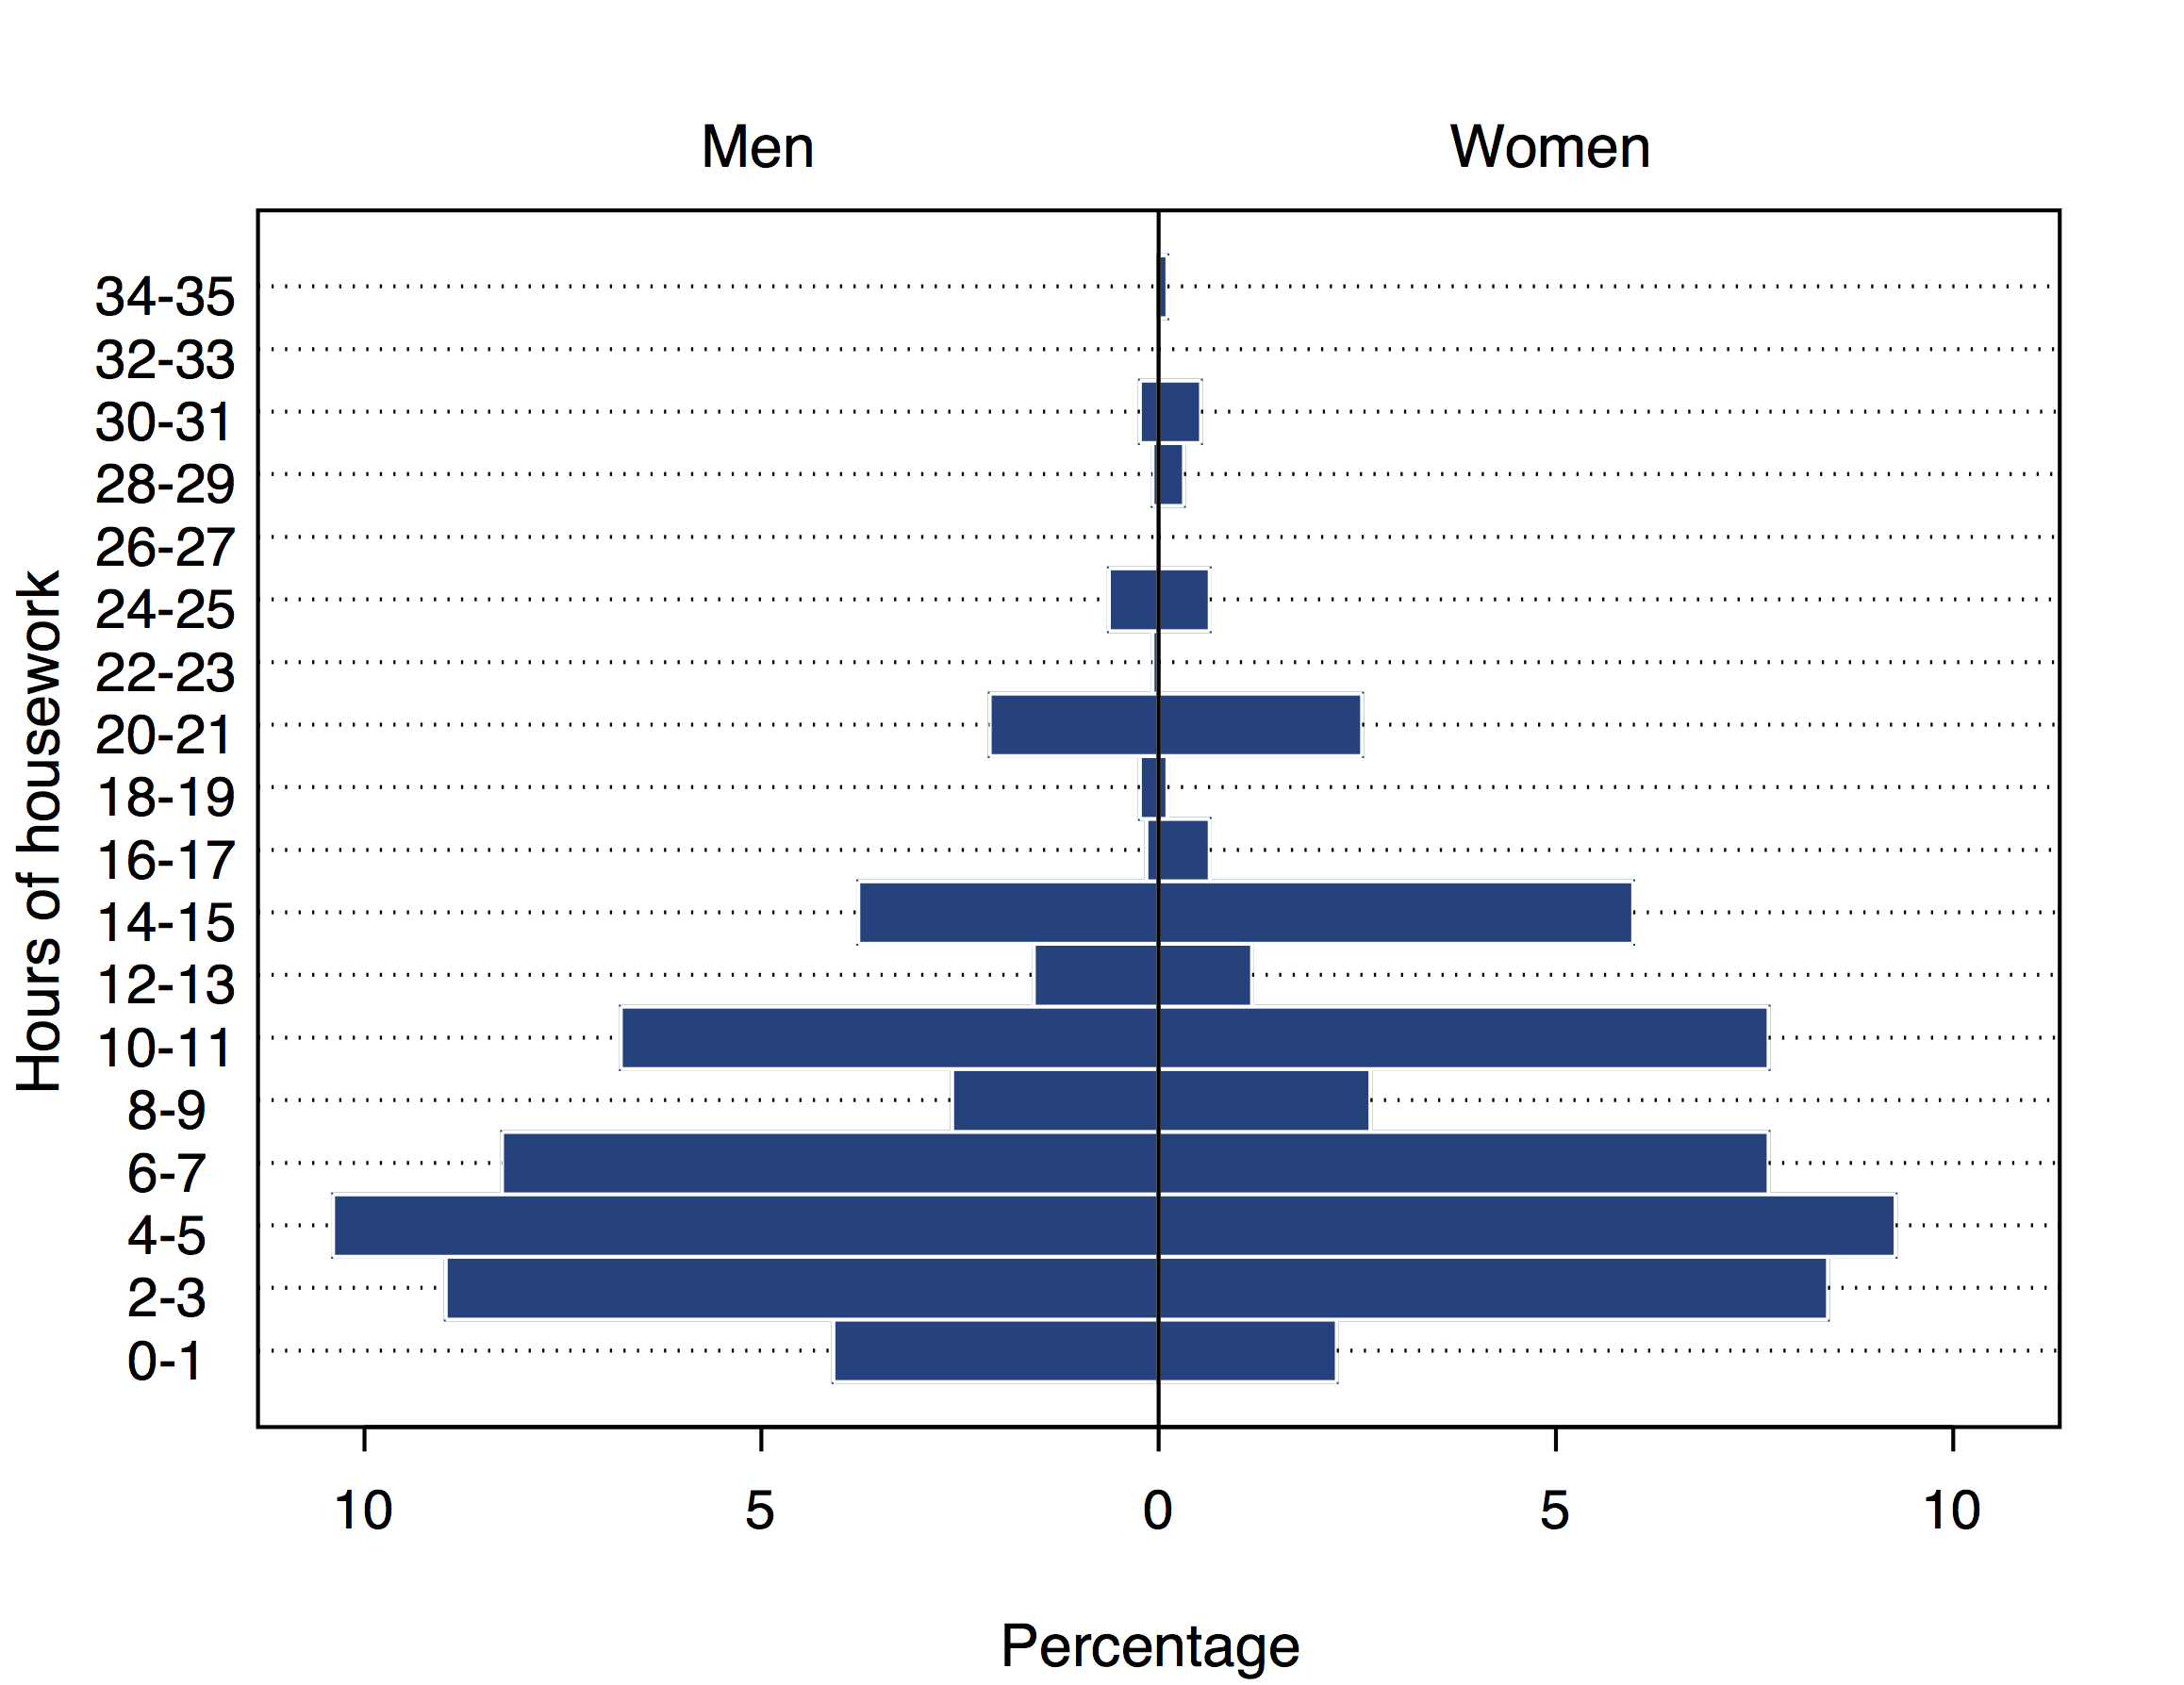
\includegraphics[width=130mm]{hworkpyramid}\\
\end{center}

\end{figure}

\begin{figure}
\caption{Frequency polygons of the sample distributions of reported
weekly hours of housework in Example 7.2, separately for men and women.
The points show the percentages of observations in the intervals of 0--3,
4--7, $\dots$, 32--35 hours (plus zero percentages at each end of
the curve).}
\label{f_hworkpolygons}
\begin{center}
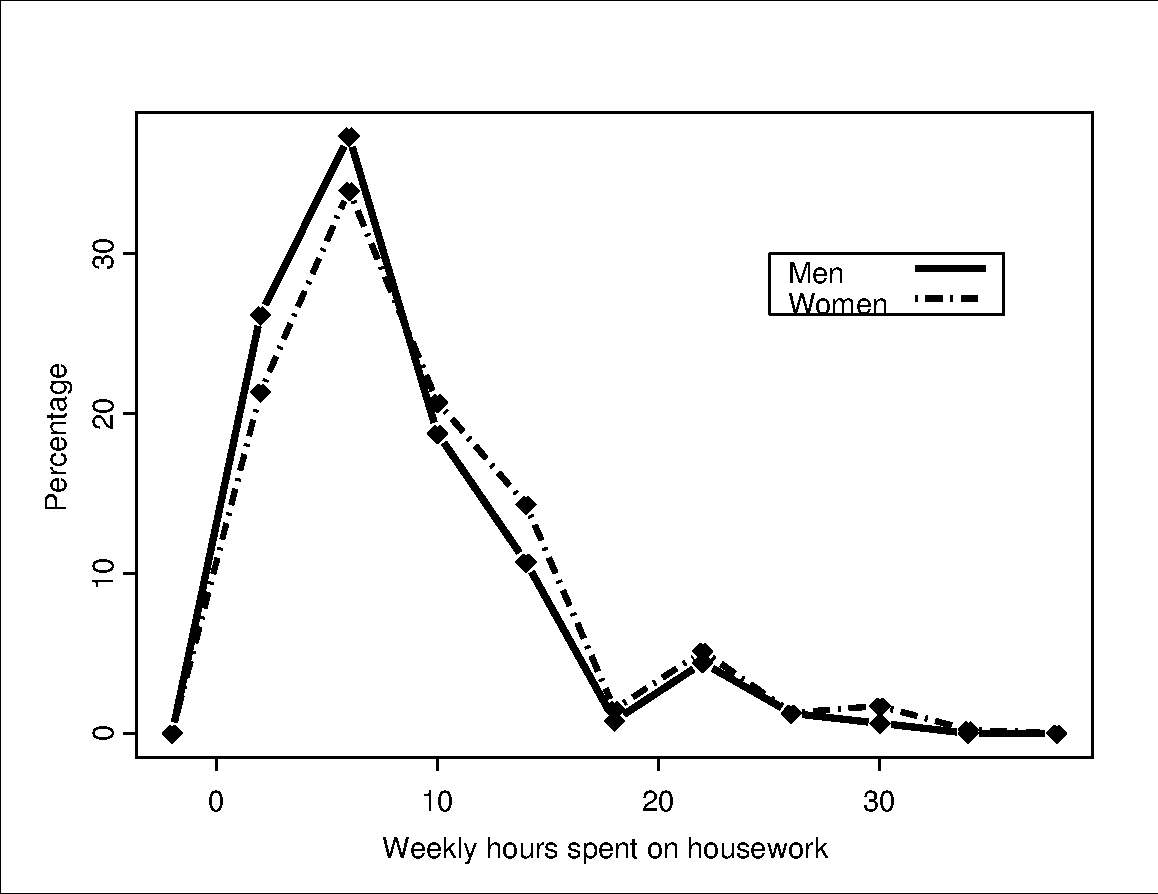
\includegraphics[width=11.5cm]{hwork}
\end{center}

\end{figure}
%\clearpage

\begin{figure}
\caption{Box plots of the sample distributions of reported
weekly hours of housework in Example 7.2, separately for men and women.}
\label{f_twoboxplots}

\begin{center}
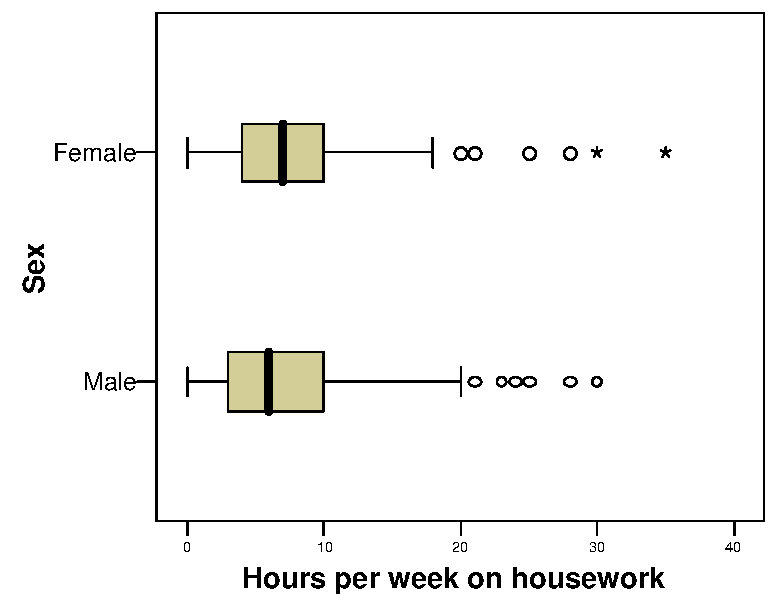
\includegraphics[width=11cm]{twoboxplots}
%\includegraphics[width=125mm]{poppolygons3}

\end{center}
\end{figure}

Figures \ref{f_hworkpyramid}--\ref{f_twoboxplots} also illustrate an
important general point about such comparisons. Typically
we focus on
comparing \emph{means} of the conditional distributions. Here the
difference between the sample means is 1.16,
i.e.\ women in the sample spend, on average, over an
hour longer on housework per week than men. The direction of the
difference could also be guessed from Figure \ref{f_hworkpolygons},
which shows that somewhat smaller proportions of women than of men
report small numbers of hours, and larger proportions of women report
large numbers. This difference will later be shown to be statistically
significant, and it is also arguably relatively large in a substantive
sense.

However, it is equally important to note that the two
distributions summarized by the graphs are nevertheless largely
similar. For example, even though the mean is higher for women, there
are clearly many women who report spending hardly any time on housework,
and many men who spend a lot of time on it. In other words, the two
distributions overlap to a large extent. This obvious point is often
somewhat neglected in public discussions of differences between groups
such as men and women or different ethnic groups. It is not uncommon to
see reports of research indicating that (say) men have higher or lower
values of something or other then women. Such statements usually refer
to differences of averages, and are often clearly important and
interesting. Less helpful, however, is the tendency to discuss the
differences almost as if the corresponding distributions had no overlap
at all, i.e.\ as if \emph{all} men were higher or lower in some
characteristic than all women. This is obviously hardly ever the case.

Box plots and frequency polygons  can also be used to compare more than
two sample distributions. For example, the experimental conditions in
the study behind Example 7.3 actually involved not only whether or not a
police officer wore sunglasses, but also whether or not he wore a gun.
Distributions of perceived friendliness given all four
combinations of these two conditions could easily be summarized by
drawing four box plots or frequency polygons in the same plot, one for
each experimental condition.

\subsection{Comparing summary statistics}
\label{ss_means_descr_tables}

Main features of sample distributions, such as their central tendencies
and variations, are described using the summary statistics introduced in
Section \ref{s_descr1_nums}. These too can be compared between groups.
Table \ref{t_groupex} shows such statistics for the examples of this
chapter. Tables like these are routinely reported for initial
description of data, even if more elaborate statistical methods are
later used.

Sometimes the association between two variables in a sample is
summarized in a single \emph{measure of association} calculated from the
data. This is especially convenient when both of the variables are
continuous (in which case the most common measure of association is
known as the \emph{correlation} coefficient). In this
section we consider as such a summary the difference
$\hat{\Delta}=\bar{Y}_{2}-\bar{Y}_{1}$ of the sample means of $Y$ in the
two groups. These differences are also shown in Table \ref{t_groupex}.

The difference of means is important because it is also the focus of the most common
methods of inference for two-group comparisons. For
purely descriptive purposes it may be as or more
convenient to report some other statistic. For example, the difference
of means of 1.16 hours in Example 7.2 could also be described in
\emph{relative} terms by saying that the women's average is about 16 per
cent higher than the men's average (because $1.16/7.33=0.158$, i.e.\ the
difference represents 15.8 \% of the men's average).

\section{Inference for two means from independent samples}
\label{s_means_inference}

\subsection{Aims of the analysis}
\label{ss_means_inference_intro}

Formulated as a statistical model in the sense discussed on page
\pageref{p_model} in Section \ref{ss_contd_probdistrs_general}, the
assumptions of the analyses considered in this section are as follows:
\begin{enumerate}
\item
\label{p_2sample}
We have a sample of $n_{1}$ independent observations of a variable $Y$
in group 1, which have a population distribution with mean $\mu_{1}$ and
standard deviation $\sigma_{1}$.
\item
We have a sample of $n_{2}$ independent observations of $Y$
in group 2, which have a population distribution with mean $\mu_{2}$ and
standard deviation $\sigma_{2}$.
\item
The two samples are independent, in the sense discussed on page
\pageref{p_depsamples}.
\item
For now, we further assume that the population standard
deviations $\sigma_{1}$ and $\sigma_{2}$ are equal, with a common value
denoted by $\sigma$.
This relatively minor assumption will be discussed
further in Section
\ref{ss_means_inference_variants}.
\end{enumerate}
We could have stated the starting points of the analyses in Chapters
\ref{c_tables} and \ref{c_probs} also in such formal terms. It is not
absolutely necessary to always do so, but we should at least remember
that any statistical analysis is based on some such
model. In particular, this helps to make it clear what our methods of
analysis do and do not assume, so that we may critically examine
whether these assumptions appear to be justified for the data at hand.

The model stated above does not require that the population
distributions of $Y$ should have the form of any particular probability
distribution. It is often further assumed that these distributions are
normal distributions, but this is not essential. Discussion of this
question is postponed until  Section \ref{ss_means_inference_variants}.

The only new term in this model statement was the ``independent'' under
assumptions 1 and 2. This statistical term can be roughly translated as
``unrelated''. The condition can usually
be regarded as satisfied when the units of analysis are different
entities, as in Examples 7.2 and 7.3 where the units within each group
are distinct individual people. In these examples the individuals in the
two groups are also distinct, from which it follows that the two \emph{samples} are independent as
required by assumption 3. The same assumption of independent
observations is also required by all of the  methods described in
Chapters \ref{c_tables} and \ref{c_probs}, although we did not state
this explicitly there.

This situation is illustrated by Example 7.2, where $Y$ is the number of hours
a person spends doing housework in a week, and the two groups are men
(group 1) and women (group 2).

The quantity of main interest is here the difference of population means
\begin{equation}
\Delta=\mu_{2}-\mu_{1}.
\label{DeltaB}
\end{equation}
In particular, if $\Delta=0$, the population means in the two groups are
the same. If $\Delta\ne 0$, they are not the same, which implies that there is an
association between $Y$ and the group in the population.

Inference on $\Delta$ can be carried out using methods which are
straightforward modifications of the ones introduced first in Chapter
\ref{c_probs}. For significance testing, the null hypothesis of interest
is
\begin{equation}
H_{0}: \; \Delta=0,
\label{mH0a}
\end{equation}
to be tested against a two-sided ($H_{a}:\; \Delta\ne 0$) or one-sided
($H_{a}:\; \Delta> 0$ or
$H_{a}:\; \Delta< 0$) alternative hypothesis. The test statistic used
to test (\ref{mH0a}) is again of the form
\begin{equation}
t=\frac{\hat{\Delta}}{\hat{\sigma}_{\hat{\Delta}}}
\label{tma}
\end{equation}
where $\hat{\Delta}$ is a sample estimate of $\Delta$, and
$\hat{\sigma}_{\hat{\Delta}}$ its estimated standard error. Here the
statistic is conventionally labelled $t$ rather than $z$ and called
the \emph{t-test statistic} because sometimes the
$t$-distribution rather than the normal is used as its sampling
distribution. This possibility is discussed in Section
\ref{ss_means_inference_variants}, and we can ignore it until then.

Confidence intervals for the differences
$\Delta$ are also of the familiar form
\begin{equation}
\hat{\Delta} \pm z_{\alpha/2}\, \hat{\sigma}_{\hat{\Delta}}
\label{ciDpa}
\end{equation}
where $z_{\alpha/2}$ is the appropriate multiplier from the standard
normal distribution to obtain the required confidence level, e.g.\
$z_{0.025}=1.96$ for 95\% confidence intervals. The multiplier is
replaced with a slightly different one if the $t$-distribution is used
as the sampling distribution, as discussed in Section
\ref{ss_means_inference_variants}.

The details of these formulas in the case of two-sample inference on
means are described next, in Section \ref{ss_means_inference_test} for
the significance test and in Section \ref{ss_means_inference_ci} for the
confidence interval.

\subsection{Significance testing: The two-sample $t$-test}
\label{ss_means_inference_test}

For tests of the difference of means
$\Delta=\mu_{2}-\mu_{1}$ between two population distributions, we
consider the null hypothesis of no difference
\begin{equation}
H_{0}: \; \Delta=0.
\label{H0m}
\end{equation}
In the
housework example, this is the hypothesis that average weekly hours of
housework in the population are the same for men and women.
It is tested against an alternative hypothesis, either the
two-sided alternative hypotheses
\begin{equation}
H_{a}: \; \Delta\ne 0
\label{Hatwom}
\end{equation}
or one of the
one-sided alternative hypotheses
\[
H_{a}:  \Delta> 0 \text{ or }

H_{a}:  \Delta< 0
\]
%\begin{eqnarray}
%H_{a}:&&  \Delta> 0 \hspace*{1.5em}\text{or}
%\label{Haonegtm}
%\\
%H_{a}:&&  \Delta < 0.
%\label{Haoneltm}
%\end{eqnarray}
In the discussion below, we concentrate on the more common two-sided
alternative.


The test statistic for testing (\ref{H0m}) is of the general form
(\ref{tma}). Here it depends on the data only through the sample means $\bar{Y}_{1}$ and $\bar{Y}_{2}$ and sample
variances $s_{1}^{2}$ and $s_{2}^{2}$ of $Y$ in the two groups.
A point estimate of $\Delta$  is
\begin{equation}
\hat{\Delta}=\bar{Y}_{2}-\bar{Y}_{1}.
\label{Dhatmu}
\end{equation}
In terms of the population parameters, the standard error of
$\hat{\Delta}$ is
\begin{equation}
\sigma_{\hat{\Delta}}=
\sqrt{\sigma^{2}_{\bar{Y}_{2}}+
\sigma^{2}_{\bar{Y}_{1}}}=
\sqrt{
\frac{\sigma^{2}_{2}}{n_{2}}+
\frac{\sigma^{2}_{1}}{n_{1}}
}.
\label{sigmaDmu}
\end{equation}
When we assume that the population standard deviations
$\sigma_{1}$ and $\sigma_{2}$ are equal, with a common value
$\sigma$, (\ref{sigmaDmu}) simplifies to
\begin{equation}
\sigma_{\hat{\Delta}} =
\sigma\; \sqrt{
\frac{1}{n_{2}}+
\frac{1}{n_{1}}
}.
\label{seDpop}
\end{equation}
The formula of the test statistic uses an estimate of this standard
error, given by
\begin{equation}
\hat{\sigma}_{\hat{\Delta}} =
\hat{\sigma} \; \sqrt{\frac{1}{n_{2}}+\frac{1}{n_{1}}}
\label{seD2}
\end{equation}
where $\hat{\sigma}$ is an estimate of $\sigma$,
calculated from
\begin{equation}
\hat{\sigma}=
\sqrt{\frac{(n_{2}-1)s^{2}_{2}+(n_{1}-1)s^{2}_{1}}{n_{1}+n_{2}-2}}.
\label{sehatjoint}
\end{equation}
Substituting (\ref{Dhatmu}) and (\ref{seD2}) into the general formula
(\ref{tma}) gives the \textbf{two-sample t-test statistic for
means}
\begin{equation}
t=
\frac{\bar{Y}_{2}-\bar{Y}_{1}}
{\hat{\sigma}\, \sqrt{1/n_{2}+1/n_{1}}}
\label{ztestmuDb}
\end{equation}
where $\hat{\sigma}$ is given by (\ref{sehatjoint}).

For an
illustration of the calculations, consider again the housework Example
7.2. Here, denoting
men by 1 and women by 2, $n_{1}=635$, $n_{2}=469$, $\bar{Y}_{1}=7.33$,
$\bar{Y}_{2}=8.49$, $s_{1}=5.53$ and $s_{2}=6.14$. The estimated mean
difference is thus
\[
\hat{\Delta}=\bar{Y}_{2}-\bar{Y}_{1}=8.49-7.33=1.16.
\]
The common value of the population standard deviation $\sigma$ is
estimated from (\ref{sehatjoint}) as
\begin{eqnarray*}
\hat{\sigma}&=&
\sqrt{\frac{(n_{2}-1)s^{2}_{2}+(n_{1}-1)s^{2}_{1}}{n_{1}+n_{2}-2}}
=
\sqrt{\frac{(469-1) 6.14^{2}+(635-1) 5.53^{2}}{635+469-2}}\\
&=& \sqrt{33.604}=5.797
\end{eqnarray*}
and the estimated standard error of $\hat{\Delta}$ is given by
(\ref{seD2}) as
\[
\hat{\sigma}_{\hat{\Delta}} =
\hat{\sigma} \; \sqrt{\frac{1}{n_{2}}+\frac{1}{n_{1}}}
=5.797 \; \sqrt{\frac{1}{469}+\frac{1}{635}}=0.353.
\]
The value of the t-test statistic (\ref{ztestmuDb}) is then obtained as
\[
t=\frac{1.16}{0.353}=3.29.
\]
These values and other quantities explained later, as well as similar
results for Example 7.3, are also shown in Table \ref{t_2testsY1}.

\begin{table}
\caption{Results of tests and confidence intervals for comparing
means for two independent samples. For Example 7.2, the difference of
means is between women and men, and for Example 7.3, it is between
wearing and not wearing sunglasses.
The test statistics and confidence intervals are obtained under the
assumption of equal population standard deviations, and
the $P$-values are for a test with a
two-sided alternative hypothesis. See the text for the
definitions of the statistics.}
\label{t_2testsY1}
\begin{center}
\begin{tabular}{|rrrrr|}\hline

$\hat{\Delta}$ &
$\hat{\sigma}_{\hat{\Delta}}$ & $t$ & $P$-value & 95 \% C.I. \\ \hline
\multicolumn{5}{|l|}{Example 7.2: Average weekly hours spent on
housework} \\
1.16 & 0.353 & 3.29 & 0.001 & (0.47; 1.85) \\  \hline
\multicolumn{5}{|l|}{Example 7.3: Perceived friendliness of a police
officer} \\
$-1.74$ & 0.383 & $-4.55$ & $<0.001$ & $(-2.49; -0.99)$
\\
\hline
\end{tabular}
\end{center}
\end{table}
%\clearpage

\label{p_spss2a}
If necessary, calculations like these can be carried out even with a
pocket calculator. It is, however, much more convenient to leave them to
statistical software. Figure \ref{f_spss2test} shows
SPSS output for the two-sample t-test for the housework data.
The first part of the table, labelled ``Group
Statistics'', shows the sample sizes $n$, means $\bar{Y}$ and standard
deviations $s$ separately for the two groups. The quantity labelled
``Std.\ Error Mean'' is $s/\sqrt{n}$. This is an estimate
of the standard error of the sample mean, which is the quantity
$\sigma/\sqrt{n}$ discussed in Section \ref{s_contd_clt}.

The second part of the table in Figure \ref{f_spss2test}, labelled
``Independent Samples Test'', gives results for the t-test itself. The
test considered here, which assumes a common population standard
deviation $\sigma$ (and thus also variance $\sigma^{2}$), is found on
the row labelled ``Equal variances assumed''. The test statistic is
shown in the column labelled ``$t$'', and the difference
$\hat{\Delta}=\bar{Y}_{2}-\bar{Y}_{1}$ and its standard error
$\hat{\sigma}_{\hat{\Delta}}$ are shown in the ``Mean Difference'' and
``Std. Error Difference'' columns respectively.
Note that the difference ($-1.16$)
has been calculated in SPSS between men and women rather than vice versa
as in Table \ref{t_2testsY1}, but this will make no difference to the
conclusions from the test.

\begin{figure}
\caption{SPSS output for a two-sample $t$-test in Example 7.2, comparing
average weekly hours spent on housework between men and women.}
\label{f_spss2test}
\begin{center}
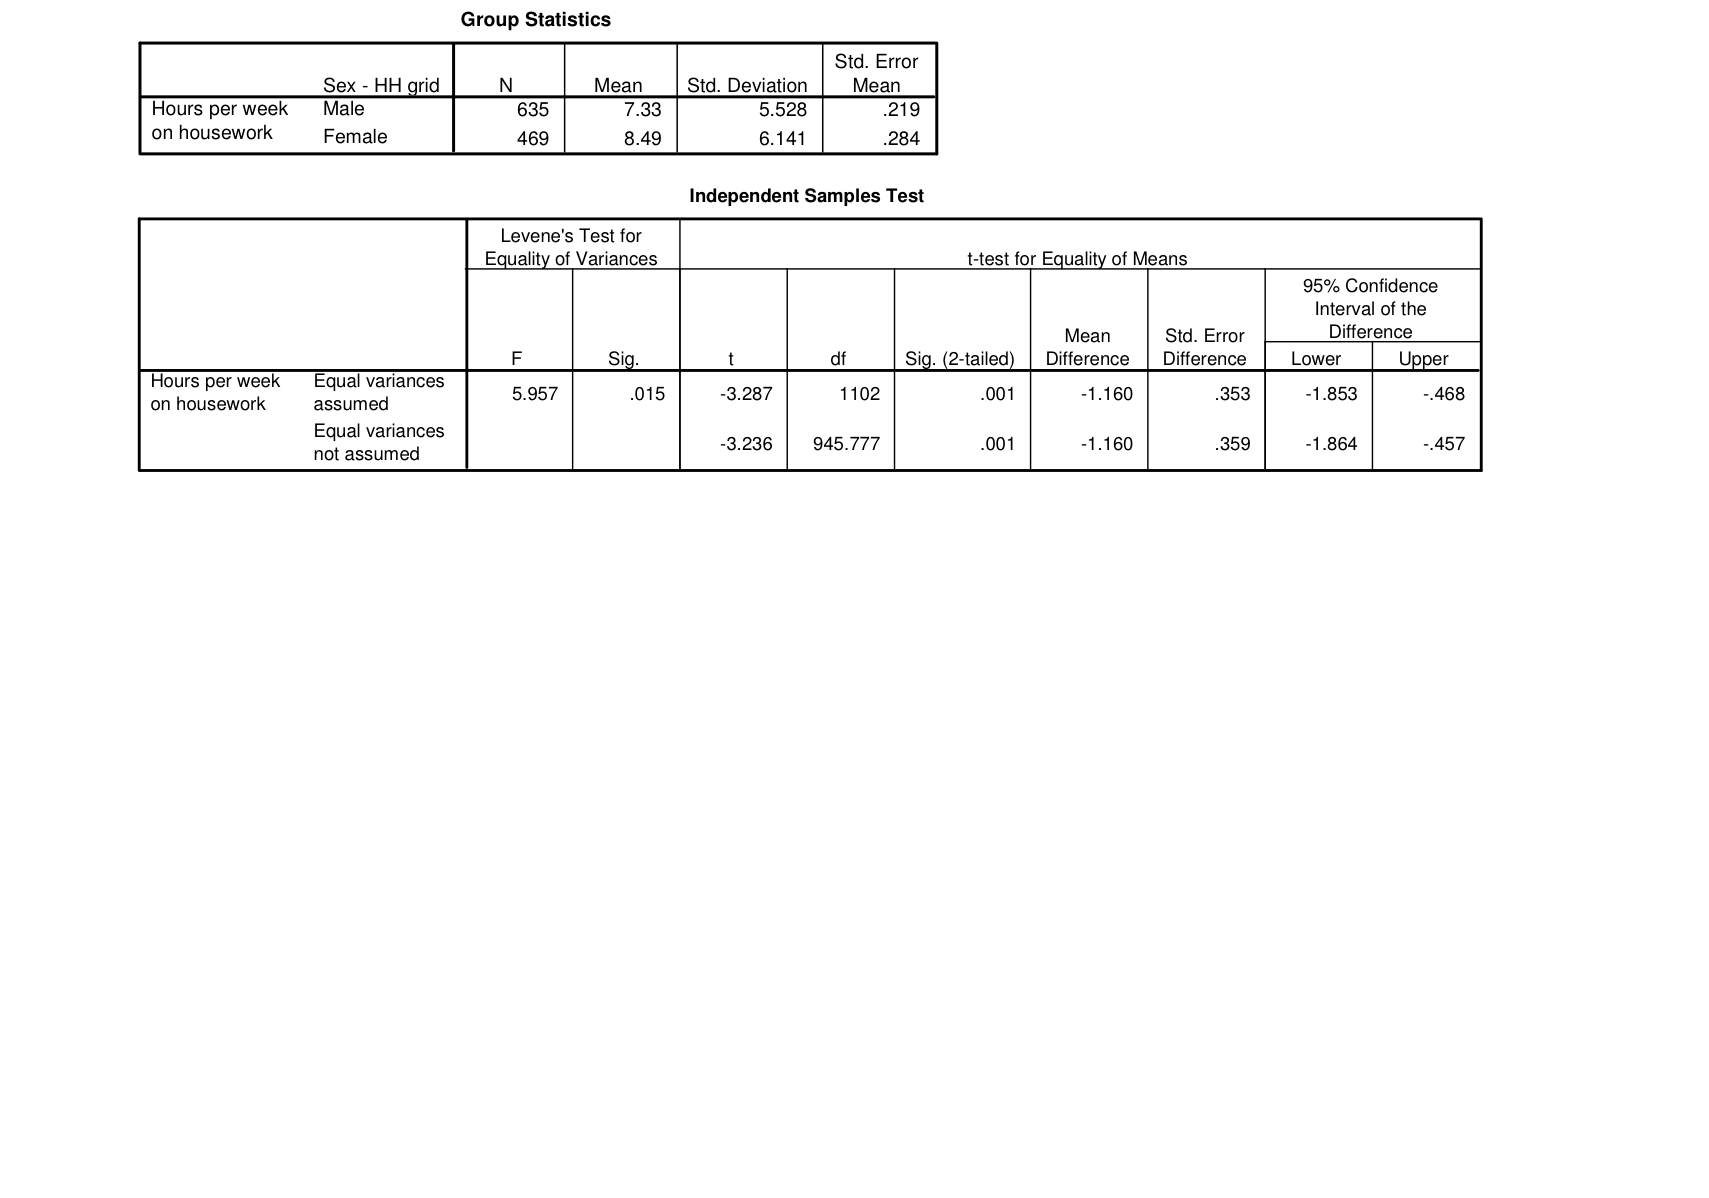
\includegraphics[bb=70 300 750 585,angle=90, height=200mm]{spss2t}
\end{center}
\end{figure}

\label{p_ztestass}
In the two-sample situation with assumptions 1--4 on page
\pageref{p_2sample}, the sampling distribution of the t-test statistic
(\ref{ztestmuDb}) is approximately a standard normal distribution
when
the null hypothesis $H_{0}: \; \Delta=\mu_{2}-\mu_{1}=0$ is true in the
population and the sample sizes are large enough.
This is again a consequence of the Central Limit Theorem. The
requirement for ``large enough'' sample sizes is fairly easy to satisfy.
A good rule of thumb is that the sample sizes $n_{1}$ and $n_{2}$ in the
two groups should both be at least 20 for the sampling distribution of
the test statistic to be well enough approximated by the standard normal
distribution. In the housework example we have data on 635 men and 469
women, so the sample sizes are clearly large enough. A variant of the test which
relaxes the condition on the sample sizes is
discussed in Section \ref{ss_means_inference_variants} below.

The $P$-value of the test is calculated from this sampling distribution
in exactly the same way as for the tests of proportions in Section
\ref{ss_probs_test1sample_samplingd}. In the housework example the value
of the $t$-test statistic is $t=3.29$. The $P$-value for testing the
null hypothesis against the two-sided alternative
(\ref{Hatwom}) is then the probability, calculated from the standard
normal distribution, of values that are at least 3.29 or at most
$-3.29$. Each of these two probabilities is about 0.0005, so the
$P$-value is $0.0005+0.0005=0.001$. In the SPSS output of Figure
\ref{f_spss2test} it is given in the
column labelled ``Sig.\ (2-tailed)'', where ``Sig.'' is short for
``significance'' and ``2-tailed'' is a synonym for ``2-sided''.

The $P$-value can also be calculated approximately using the table of
the standard normal distribution (see Table \ref{t_ttable} on page
\pageref{t_ttable}), as explained in Section
\ref{ss_probs_test1sample_samplingd}. Here the test statistic $t=3.29$,
which is larger than the critical values 1.65, 1.96 and 2.58 for the
0.10, 0.05 and 0.01 significance levels for a two-sided test, so we can
report that $P<0.01$. Here $t$ is by chance actually equal (to two
decimal places) to the critical value for the 0.001 significance level,
so we could also report $P=0.001$. These findings agree, as they should,
with the exact $P$-value of 0.001 shown in the SPSS output.

In conclusion, the two-sample $t$-test in Example 7.2 indicates that there
is very strong evidence (with $P=0.001$ for the two-sided test) against
the claim that the hours of weekly housework are on average the
same for men and women in the population.

Here we showed raw SPSS output in Figure \ref{f_spss2test} because we
wanted to explain its contents
and format. Note, however, that such unedited computer output is
rarely if ever appropriate in research reports.
Instead, results of statistical analyses should be given in text or
tables formatted in appropriate ways for presentation. See Table
\ref{t_2testsY1} and various other examples in this coursepack and
textbooks on statistics.


\newpage
To summarise the elements of the test again, we repeat them briefly, now
for Example 7.3, the experiment on the effect of eye
contact on the perceived friendliness of police officers (c.f.\ Table
\ref{t_groupex} on page \pageref{t_groupex} for the summary statistics):
\begin{enumerate}
\item
Data: samples from two groups,
one with the experimental condition where
the officer wore no sunglasses,
with sample size $n_{1}=67$, mean $\bar{Y}_{1}=8.23$ and standard
deviation $s_{1}=2.39$, and
the second with the experimental condition where
the officer did wear sunglasses,
with $n_{2}=66$, $\bar{Y}_{2}=6.49$ and $s_{2}=2.01$.
\item
Assumptions: the observations are random samples of statistically
independent observations from two populations, one
with mean $\mu_{1}$ and standard deviation
$\sigma_{1}$, and the other with
with mean $\mu_{2}$ and the same standard deviation
$\sigma_{2}$, where the standard deviations are equal, with value
$\sigma=\sigma_{1}=\sigma_{2}$. The sample sizes $n_{1}$ and $n_{2}$ are
sufficiently large, say
both at least 20, for the sampling distribution of the test statistic
under the null hypothesis to be approximately standard normal.
\item
Hypotheses: These are about the difference of the population means
$\Delta=\mu_{2}-\mu_{1}$, with
null hypothesis $H_{0}: \Delta=0$. The two-sided alternative
hypothesis $H_{a}: \Delta\ne 0$ is considered in this example.
\item
The test statistic: the two-sample $t$-statistic
\[
t=\frac{\hat{\Delta}}{\hat{\sigma}_{\hat{\Delta}}}=
\frac{-1.74}{0.383}=-4.55
\]
where
\[
\hat{\Delta}=\bar{Y}_{2}-\bar{Y}_{1}=6.49-8.23=-1.74
\]
and
\[
\hat{\sigma}_{\hat{\Delta}}=
\hat{\sigma} \; \sqrt{\frac{1}{n_{2}}+\frac{1}{n_{1}}}
=2.210 \times \sqrt{
\frac{1}{66}+\frac{1}{67}}=0.383
\]
with
\[
\hat{\sigma}=
\sqrt{\frac{(n_{2}-1)s^{2}_{2}+(n_{1}-1)s^{2}_{1}}{n_{1}+n_{2}-2}}
=
\sqrt{\frac{65\times 2.01^{2}+66\times 2.39^{2}}{131}}
=2.210
\]
\item
The sampling distribution of the test statistic when $H_{0}$ is true:
approximately the standard normal distribution.
\item
The $P$-value: the probability that a randomly selected value from the
standard normal distribution is at most $-4.55$ or at least 4.55, which is
about 0.000005 (reported as $P<0.001$).
\item
Conclusion: A two-sample
$t$-test indicates very strong evidence that the average perceived
level of the friendliness of a police officer is different when the
officer is wearing reflective sunglasses than when the officer is not
wearing such glasses ($P<0.001$).
\end{enumerate}

\newpage
\subsection{Confidence intervals for a difference of two means}
\label{ss_means_inference_ci}

A confidence interval for the mean difference $\Delta=\mu_{1}-\mu_{2}$
is obtained by substituting appropriate expressions into the general
formula (\ref{ciDpa}). Specifically, here
$\hat{\Delta}=\bar{Y}_{2}-\bar{Y}_{1}$ and a 95\% confidence interval
for $\Delta$ is
\begin{equation}
(\bar{Y}_{2}-\bar{Y}_{1}) \pm 1.96\;  \hat{\sigma} \;
\sqrt{
\frac{1}{n_{2}}+\frac{1}{n_{1}}
}
\label{ciDmu2}
\end{equation}
where $\hat{\sigma}$ is obtained from equation \ref{sehatjoint}.
The validity of this again requires that the sample sizes $n_{1}$ and $n_{2}$ from both
groups are reasonably large, say both at least 20.
For the housework Example 7.2, the 95\% confidence interval is
\[
1.16\pm 1.96\times 0.353 = 1.16 \pm 0.69 = (0.47; 1.85)
\]
using the values of $\bar{Y}_{2}-\bar{Y}_{1}$ and its standard error
calculated earlier.
This interval is
also shown in Table \ref{t_2testsY1} on page \pageref{t_2testsY1} and in
the SPSS output in Figure \ref{f_spss2test} on page
\pageref{f_spss2test}\label{p_spss2c}.
In the latter, the interval is given as (-1.85; -0.47)
because it is expressed for the difference defined in
the opposite direction (men $-$ women instead of vice versa).
For Example 7.3, the 95\% confidence interval is $-1.74\pm 1.96\times 0.383=(-2.49;
-0.99)$.


Based on the data in Example 7.2 we are thus 95 \% confident that the
difference between women's and men's average hours of reported weekly
housework in the population is between 0.47 and 1.85 hours. In
substantive terms this interval, from just under half an hour to nearly
two hours, is arguably fairly wide in that its two end points might well
be regarded as substantially different from each other. The difference
between women's and men's average housework hours is thus estimated
fairly imprecisely from this survey.


\subsection{Variants of the test and confidence interval}
\label{ss_means_inference_variants}

\subsubsection{Allowing unequal population variances}

The two-sample $t$-test and confidence interval for the difference of
means were stated above under the assumption that the standard
deviations $\sigma_{1}$ and $\sigma_{2}$ of the variable of interest $Y$
are the same in both of the two groups being compared. This
assumption is not in fact essential. If it is omitted, we obtain
formulas which differ from the ones discussed above only in one part of
the calculations.

Suppose that we do allow the unknown values of $\sigma_{1}$ and $\sigma_{2}$ to be
different from each other. In other words, we consider the model stated
on page \pageref{p_2sample}, without assumption 4 that
$\sigma_{1}=\sigma_{2}$. The test
statistic is then still of the same form as before, i.e.\
$t=\hat{\Delta}/\hat{\sigma}_{\hat{\Delta}}$, with
$\hat{\Delta}=\bar{Y}_{2}-\bar{Y}_{1}$. The only change in the
calculations is that the estimate of the standard error of $\hat{\Delta}$, the formula
of which is given by equation (\ref{sigmaDmu}) on page
\pageref{sigmaDmu},  now uses separate estimates of $\sigma_{1}$ and
$\sigma_{2}$. The obvious choices for these are the
corresponding sample standard deviations, $s_{1}$ for $\sigma_{1}$ and
$s_{2}$ for $\sigma_{2}$. This gives the estimated standard error as
\begin{equation}
\hat{\sigma}_{\hat{\Delta}}=
\sqrt{
\frac{s_{2}^{2}}{n_{2}}+
\frac{s_{1}^{2}}{n_{1}}
}.
\label{seDmu_ne}
\end{equation}
Substituting this to the formula of the test statistic yields the
two-sample $t$-test statistic without the assumption of equal population
standard deviations,
\begin{equation}
t=
\frac{\bar{Y}_{2}-\bar{Y}_{1}}
{\sqrt{s^{2}_{2}/n_{2}+s^{2}_{1}/n_{1}}}.
\label{ztestmuD}
\end{equation}
The sampling distribution of this under the null hypothesis is again
approximately a standard normal distribution when the sample sizes
$n_{1}$ and $n_{2}$ are both at least 20. The $P$-value for the test is
obtained in exactly the same way as before, and the
principles of interpreting the result of the test are also
unchanged.

For the confidence interval, the only change from Section
\ref{ss_means_inference_ci} is again that the estimated standard error
is changed, so for a 95\% confidence interval we use
\begin{equation}
(\bar{Y}_{2}-\bar{Y}_{1}) \pm 1.96 \;
\sqrt{
\frac{s^{2}_{2}}{n_{2}}+\frac{s^{2}_{1}}{n_{1}}
}.
\label{ciDmu}
\end{equation}


In the housework example 7.2, the estimated standard error (\ref{seDmu_ne}) is
\[
\hat{\sigma}_{\hat{\Delta}}=
\sqrt{
\frac{6.14^{2}}{469}+
\frac{5.53^{2}}{635}
}=
\sqrt{0.1285}=0.359,
\]
the value of the test statistic is
\[
t=\frac{1.16}{0.359}=3.23,
\]
and the two-sided $P$-value is now $P=0.001$. Recall that
when the population standard deviations
were assumed to be equal, we obtained
$\hat{\sigma}_{\hat{\Delta}}=0.353$, $t=3.29$ and again $P=0.001$. The
two sets of results are thus very similar, and the conclusions from the
test are the same in both cases. The differences between the two
variants of the test are even smaller in Example 7.3, where the
estimated standard error $\hat{\sigma}_{\hat{\Delta}}=0.383$ is the same
(to three decimal places) in both cases, and the results are thus
identical\footnote{In this case this is a consquence of the fact that
the sample sizes (67 and 66) in the two groups are very similar. When
they are exactly equal, formulas
(\ref{sehatjoint})--(\ref{ztestmuDb}) and (\ref{seDmu_ne}) actually give
exactly the same value for the standard error
$\hat{\sigma}_{\hat{\Delta}}$, and $t$ is thus also the same for both
variants of the test.
}. In both examples the confidence intervals obtained
from (\ref{ciDmu2}) and (\ref{ciDmu}) are also very similar.
Both variants of the two-sample analyses are shown in SPSS output (c.f.\
Figure \ref{f_spss2test} on page \pageref{f_spss2test}), the ones
assuming equal population standard deviations on the row labelled
``Equal variances assumed'' and the one without this assumption on the
``Equal variances not assumed'' row\footnote{The output also shows,
under ``Levene's test'', a test statistic and $P$-value for testing the
hypothesis of equal standard deviations ($H_{0}: \,
\sigma_{1}=\sigma_{2}$). However, we prefer not to rely on this because
the test requires the additional assumption that the population
distributions are normal, and is very sensitive to the correctness of
this assumption.}.

Which methods should we then use, the ones with or without the assumption of
equal population variances? In practice the choice rarely makes much
difference, and the $P$-values and conclusions from the two versions of
the test are typically very similar\footnote{In the MY451 examination
and homework, for example, both variants of the test are equally
acceptable, unless a question explicitly states otherwise.}.
Not assuming the variances to be equal
has the advantage of making fewer restrictive assumptions about the
population. For
this reason it should be used in the rare cases where the $P$-values
obtained under the different assumptions are substantially different.
This version of the test statistic is also slightly easier to calculate
by hand, since (\ref{seDmu_ne}) is a slightly simpler formula than
(\ref{seD2})--(\ref{sehatjoint}). On the other hand, the test statistic
which does assume equal standard deviations has the advantage that it is
more closely related to analogous tests used in more general contexts
(especially the method of linear regression modelling, discussed in Chapter
\ref{c_regression}). It is also preferable when the sample
sizes are very small, as discussed below.


\subsubsection{Using the $t$ distribution}

As discussed in Section \ref{s_contd_probdistrs}, it is often assumed
that the population distributions of the variables under consideration
are described by particular probability distributions. In this chapter,
however, such assumptions have so far been avoided. This is a
consequence of the Central Limit Theorem, which ensures that as long as
the sample sizes are large enough, the sampling distribution of the
two-sample $t$-test statistic is approximately the standard normal
distribution, irrespective of the forms of the population distributions
of $Y$ in the two groups. In this section we briefly describe variants
of the test and confidence interval which \emph{do} assume that the
population distributions are of a particular form, specifically that
they are normal distributions. This changes the sampling distribution
that is used for the test statistic and for the multiplier of the
confidence interval, but the analyses are otherwise unchanged.

For the significance test, there are again two variants depending on the assumptions about the the population standard
deviations $\sigma_{1}$ and $\sigma_{2}$. Consider first the case
where these are assumed to be
equal. The sampling distribution is then given by the following result,
which now holds for \emph{any} sample sizes $n_{1}$ and $n_{2}$:
\begin{itemize}
\item
In the two-sample situation specified by assumptions 1--4 on page
\pageref{p_2sample} (including the assumption of
equal population standard deviations,
$\sigma_{1}=\sigma_{2}=\sigma$), and if also the distribution of $Y$ is
a normal distribution in both groups, the sampling distribution of the
t-test statistic (\ref{ztestmuDb}) is a $t$ distribution with
$n_{1}+n_{2}-2$ degrees of freedom when the null hypothesis $H_{0}: \;
\Delta=\mu_{2}-\mu_{1}=0$ is true in the population.
\end{itemize}
The $\mathbf{t}$ \textbf{distributions} mentioned in this result are a
family of distributions with different degrees of freedom, in a similar
way as the $\chi^{2}$ distributions discussed in Section
\ref{ss_tables_chi2test_sdist}. All $t$
distributions are symmetric around 0.
Their
shape is quite similar to that of the standard normal distribution,
except that the variance of
a $t$ distribution is somewhat larger and its tails thus heavier.
The difference is noticeable only
when the degrees of freedom are small, as seen in Figure
\ref{f_tdistr1}. This shows the curves for the $t$ distributions with 6
and 30 degrees of freedom, compared to the standard normal distribution.
It can be seen that the $t_{30}$ distribution is already very similar to
the $N(0,1)$ distribution. With degrees of freedom larger than about 30,
the difference becomes almost indistinguishable.

\begin{figure}
\caption{
Curves of two $t$ distributions with small degrees of freedom, compared
to the standard normal distribution.
}
\label{f_tdistr1}
\begin{center}

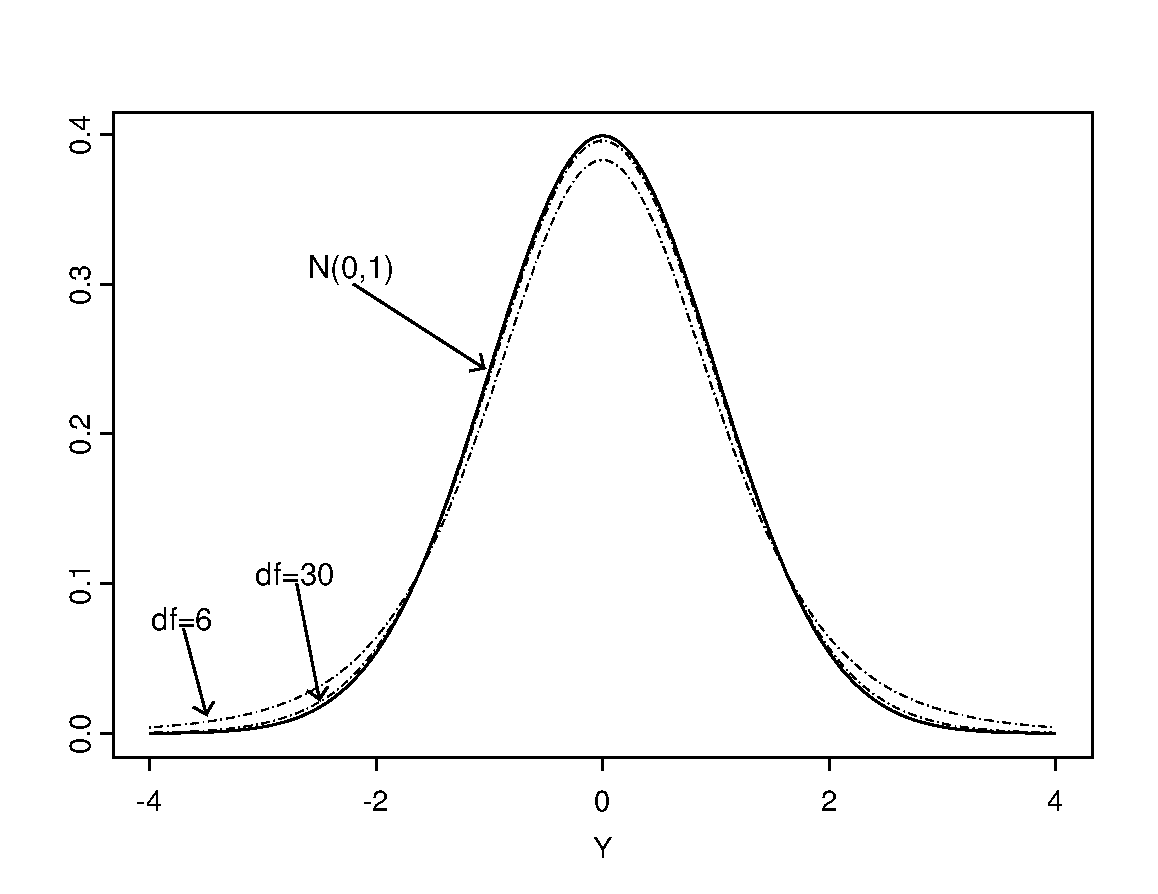
\includegraphics[width=13cm]{tdistr1}
\end{center}

\end{figure}

If we use this result for the test, the
$P$-value is obtained from the $t$ distribution with $n_{1}+n_{2}-2$
degrees of freedom (often denoted $t_{n1+n2-2}$).
The principles of doing this are exactly the
same as those described in Section
\ref{ss_probs_test1sample_samplingd}, and
can be graphically illustrated by plots similar to those in Figure
\ref{f_pval_prob} on page
\pageref{f_pval_prob}.
Precise $P$-values are again
obtained using a computer. In fact, $P$-values in SPSS output for the
two-sample $t$-test (c.f.\ Figure \ref{f_spss2test} on page
\pageref{f_spss2test}) are actually those obtained from the $t$
distribution (with the degrees of freedom shown in the column labelled
``df'') rather than the standard normal distribution.
Differences between the two are, however, very small if the sample sizes are even
moderately large, because then the degrees of freedom $df=n_{1}+n_{2}-2$
are large enough for the two distributions to be virtually identical.
This is the case, for instance, in both
of the examples considered so far in this chapter, where $df=1102$ in
Example 7.2 and $df=131$ in Example 7.3.

If precise $P$-values from the $t$ distribution are not available,
upper bounds for them can again be obtained using appropriate tables, in
the same way as in Section
\ref{ss_probs_test1sample_samplingd}. Now, however,
the critical values depend also on the degrees of freedom. Because of
this, introductory text books on statistics typically include a
table of critical values for $t$ distributions for a selection of
degrees of freedom. A table of this kind is shown on page
\pageref{s_disttables_t} at the end of this course pack. Each row of the
table corresponds to a $t$ distribution with the degrees of freedom
given in the column labelled ``df''. As here, such tables
typically include all degrees of freedom between 1 and 30, plus
a selection of larger values, here 40, 60 and 120.

The last row is labelled ``$\infty$'', the mathematical symbol for
infinity. This corresponds to the standard normal distribution, as a $t$
distribution with infinite degrees of freedom is equal to the standard normal. The practical implication of this is that
the standard normal distribution is a good enough approximation for any
$t$ distribution with reasonably large degrees of freedom. The table
thus lists individual degrees of freedom only up to some point, and the
last row will be used for any values larger than this. For
degrees of freedom between two values shown in the table (e.g.\ 50 when
only 40 and 60 are given), it is best to use the values for the nearest
available degrees of freedom \emph{below} the required ones (e.g.\ use
40 for 50). This will give a ``conservative'' approximate
$P$-value which may be slightly larger than the exact value.

As for the standard normal distribution, the table is used to identify
critical values for different significance levels (c.f.\ the information
in Table \ref{t_ttable}). For example, if the degrees of freedom are 20,
the critical value for two-sided tests at the significance level 0.05 in
the ``0.025'' column on the row labelled ``20''. This is 2.086. In
general, critical values for $t$ distributions are somewhat larger than
corresponding values for the standard normal distribution, but the
difference between the two is quite small when the degrees of freedom
are reasonably large.


The $t$-test and the $t$ distribution are among the oldest tools of
statistical inference. They were introduced in 1908 by W.\ S.\
Gosset\footnote{Student (1908). ``The probable error of a mean''.
\emph{Biometrika} \textbf{6}, 1--25.}, initially for the one-sample case
discussed in Section \ref{s_means_1sample}. Gosset was working as a
chemist at the Guinness brewery at St.\ James' Gate, Dublin. He
published his findings under the pseudonym ``Student'', and the
distribution is often known as \emph{Student's $t$ distribution}.

These results for the sampling distribution hold when the
population standard deviations $\sigma_{1}$ and $\sigma_{2}$ are assumed
to be equal. If this assumption is not made, the test statistic is again
calculated using formulas (\ref{seDmu_ne}) and (\ref{ztestmuD}) on
page \pageref{ztestmuD}. This case is mathematically more difficult than
the previous one, because
the sampling distribution of the test statistic under the null
hypothesis is then not exactly a $t$ distribution even when the
population distributions are normal. One way of dealing with this
complication (which is known as the Behrens--Fisher problem) is
to find a $t$ distribution which is a good approximation of the true
sampling distribution. The degrees of freedom of this approximating
distribution are given by
\begin{equation}
df=\frac{\left(
\frac{s^{2}_{1}}{n_{1}}+
\frac{s^{2}_{2}}{n_{2}}
\right)^{2}}
{
\left(\frac{s_{1}^{2}}{n_{1}}\right)^{2}\;
\left(\frac{1}{n_{1}-1}\right)
+
\left(\frac{s_{2}^{2}}{n_{2}}\right)^{2}\;
\left(\frac{1}{n_{2}-1}\right)
}.
\label{satter_df}
\end{equation}
This formula, which is known as the Welch-Satterthwaite approximation,
is not particularly interesting or worth learning in itself. It is
presented here purely for completeness, and to give an idea of how the
degrees of freedom given in the SPSS output are obtained. In Example 7.2
(see Figure \ref{f_spss2test} on page \pageref{f_spss2test}) these
degrees of freedom are 945.777, showing that the approximate degrees of
freedom from (\ref{satter_df}) are often not whole numbers. If
approximate $P$-values are then obtained from a $t$-table, we need to
use values for the nearest whole-number degrees of freedom shown in the
table. This problem does not arise if the calculations are done with a
computer.

Two sample $t$-test statistics (in two variants, under equal and unequal
population standard deviations) have now been defined under two different
sets of assumptions about the population distributions.
In each case, the formula of the test statistic is
the same, so the only difference is in the form of its sampling
distribution under the null hypothesis. If the population distributions
of $Y$ in the two groups are assumed to be normal, the sampling
distribution of the $t$-statistic is a $t$ distribution with appropriate
degrees of freedom. If the sample sizes are reasonably large, the
sampling distribution is approximately standard normal, whatever the
shape of the population distribution. Which set of assumptions should we
then use? The following guidelines can be used to make the
choice:
\begin{itemize}
\item
The easiest and arguably most common case is the one where both sample
sizes $n_{1}$ and $n_{2}$ are large enough (both greater than 20, say)
for the standard normal approximation of the sampling distribution to be
reasonably accurate. Because the degrees of freedom of the appropriate
$t$ distribution are then also large, the two sampling distributions are
very similar, and conclusions from the test will be similar in either
case. It is then
purely a matter of convenience which sampling distribution is used:
\begin{itemize}
\item
If you use a computer (e.g.\ SPSS) to carry out the test or you are
(e.g.\ in an exam) given computer output, use the $P$-value in the
output. This will be from the $t$ distribution.
\item
If you need to calculate the test statistic by hand and thus need to use
tables of critical values to draw the conclusion, use the critical
values for the standard normal distribution (see Table \ref{t_ttable}).
\end{itemize}
\item
When the sample sizes are small (e.g.\ if one or both of them are less
than 20), only the $t$ distribution can be used, and even then only
if $Y$ is approximately normally
distributed in both groups in the population.
For some variables
(say weight or blood pressure) we might have some confidence that this
is the case, perhaps from previous, larger studies. In other cases
the normality of $Y$ can only be assessed based on its sample
distribution, which of course is not very informative when the sample is
small. In most cases, some doubt will remain, so the results of a
$t$-test from small samples should be treated with caution. An
alternative is then to use \emph{nonparametric} tests which avoid the
assumption of normality, for example the so-called Wilcoxon--Mann--Whitney test.
These, however,
are not covered on
this course.
\end{itemize}
There are also situations where the population distribution of $Y$
cannot possibly be normal, so the possibility of referring to a $t$
distribution does not arise. One example are the tests on population
proportions that were discussed in Chapter \ref{c_probs}. There the only
possibility we discussed was to use the approximate standard normal
sampling distribution, as long as the sample sizes were large enough.
Because the $t$-distribution is never relevant there, the test statistic
is conventionally called the $z$-test statistic rather than $t$.
Sometimes the label $z$ instead of $t$ is used also for two-sample
$t$-statistics described in this chapter. This does not change the test
itself.


It is also possible to obtain a confidence interval for $\Delta$ which
is valid for even very small sample sizes $n_{1}$ and $n_{2}$, but only
under the further assumption that the population distribution of $Y$ in
both groups is normal. This affects only the multiplier
of the standard errors, which is now based on a $t$ distribution. The appropriate degrees of
freedom are again $df=n_{1}+n_{2}-2$ when the population standard
deviations are assumed equal, and approximately given by equation
(\ref{satter_df}) if not. In this case the multiplier in (\ref{ciDpa})
may be labelled $t^{(df)}_{\alpha/2}$ instead of $z_{\alpha/2}$ to draw
attention to the fact that it comes from a $t$-distribution and
depends on the degrees of freedom $df$ as well as
the significance level $1-\alpha$.

Any multiplier $t_{\alpha/2}^{(df)}$ is obtained from the relevant $t$
distribution using exactly the same logic as the one explained for the
normal distribution in the previous section, using a computer or a table
of $t$ distributions. For example, in the $t$ table on page
\pageref{s_disttables_t}, multipliers for a 95\% confidence interval are
the numbers given in the column labelled ``0.025''. Suppose, for
instance, that the sample sizes $n_{1}$ and $n_{2}$ are both 10 and
population standard deviations are assumed equal, so that
$df=10+10-2=18$. The table shows that a $t$-based 95\% confidence
interval would then use the multiplier 2.101. This is somewhat larger
than the corresponding multiplier 1.96 from the normal distribution, and
the $t$-based interval is somewhat wider than one based on the normal
distribution. The difference between the two becomes very small when the
sample sizes are even moderately large, because then $df$ is large and
$t_{\alpha/2}^{(df)}$ is very close to 1.96.

The choice between confidence intervals based on the normal or a $t$
distribution involves the same considerations
as for the significance test.
In short, if the sample sizes are not very
small, the choice makes little difference and can be based on
convenience. If you are calculating an interval by hand, a normal-based
one is easier to use because the multiplier (e.g.\ 1.96 for 95\%
intervals) does not depend on the sample sizes. If, instead,
a computer is used, it typically gives confidence intervals for differences
of means based on the $t$ distribution, so these are easier to use.
Finally, if one or both of the sample sizes are small, only $t$-based
intervals can safely be used, and then only if you are confident that
the population distributions of $Y$  are approximately normal.


%\renewcommand{\thefootnote}{\fnsymbol{footnote}}
\section{Tests and confidence intervals for a single
mean}
%\footnote[1]{The material of this section is not required in the
%examination.}}
\label{s_means_1sample}
%\renewcommand{\thefootnote}{\arabic{footnote}}

The task considered in this section is inference on the population mean
of a continuous, interval-level variable $Y$ in a single population.
This is thus analogous to the analysis of a single proportion in
Sections \ref{s_probs_test1sample}--\ref{s_probs_1sampleci}, but with a
continuous variable of interest.

We use Example 7.1 on survey data on diet for illustration. We will
consider two variables, daily consumption of portions of fruit and
vegetables, and the percentage of total faily energy intake obtained
from fat and fatty acids. These will be analysed separately, each in
turn in the role of the variable of interest $Y$. Summary statistics for
the variables are shown in Table \ref{t_ttests1}

\begin{table}
\caption{Summary statistics, $t$-tests and confidence intervals
for the mean for the two variables in Example 7.1
(variables from the Diet and Nutrition Survey).}
\label{t_ttests1}
\begin{center}
\begin{tabular}{|l|rrr|rrrr|c|}\hline
 & & & & & &\multicolumn{2}{c|}{$P$-value} & \\
  & & & & & & Two-& One- & 95\% CI \\
Variable&   $n$ & $\bar{Y}$ & $s$ & $\mu_{0}$ & $t$ & sided$^{*}$
& sided$^{\dagger}$ & for $\mu$\\
\hline
Fruit and vegetable & 1724 & 2.8 & 2.15
& 5 & -49.49 & $<0.001$&
$<0.001$& (2.70; 2.90)\\
consumption &  & & & & & & & \\
(400g portions)  & &  & & & & & & \\
Total energy intake & 1724 & 35.3& 6.11 & 35 & 2.04 & 0.042 &
0.021 & (35.01; 35.59)\\
from fat (\%) & & & & & &  & & \\
\hline
\multicolumn{9}{l}{{\footnotesize $n=$sample size; $\bar{Y}=$sample
mean; $s=$sample standard deviation
}}\\
\multicolumn{9}{l}{{\footnotesize$\mu_{0}=$null hypothesis about the
population mean; $t=t$-test statistic}}\\
\multicolumn{9}{l}{{\footnotesize $*$: Alternative hypothesis $H_{a}:
\mu\ne \mu_{0}$}}\\
\multicolumn{9}{l}{{\footnotesize $\dagger$: Alternative hypotheses $H_{a}:
\mu<5$ and $\mu>35$ respectively}}
\end{tabular}
\end{center}
\end{table}

The setting for the analysis of this section is summarised as a
statistical model for observations of a variable $Y$ as follows:
\begin{enumerate}
\item
The population distribution of
$Y$ has some unknown mean $\mu$ and unknown standard deviation $\sigma$.
\item
The observations $Y_{1}, Y_{2}, \dots, Y_{n}$ in the sample are a
random sample from the population.
\item
The observations are statistically independent,
as discussed on
page \pageref{p_2sample}.
\end{enumerate}
It is not necessary to assume that the population distribution
has a particular form. However, this is again sometimes assumed to be a normal
distribution, in which case the analyses may be modified in ways
discussed below.

The only quantity of interest considered here is $\mu$, the population
mean of $Y$. In the diet examples this is the mean number of portions of
fruit and vegetables, or mean percentage of energy derived from fat
(both on an average day for an individual) among the members of the
population (which for this survey is British adults aged
19--64).

Because no separate groups are being compared, questions of interest are
now not about differences between different group means, but about the
value of $\mu$ itself. The best single estimate (\emph{point estimate})
of $\mu$ is the sample mean $\bar{Y}$. More information is provided by a
confidence interval which shows
which values of $\mu$ are plausible given the observed data.

Significance testing focuses on the question of
whether it is plausible that the true value of $\mu$ is equal to a
particular value $\mu_{0}$ specified by the researcher. The specific
value of $\mu_{0}$ to be tested is suggested by the research questions.
For example, we will consider $\mu_{0}=5$
for portions of fruit and vegetables and $\mu_{0}=35$ for the percentage
of energy from fat. These values are chosen because they correspond to
recommendations by the Department of Health that we should consume at
least 5 portions of fruit and vegetables a day, and that fat should
contribute no more than 35\% of total energy intake. The statistical
question is thus whether the average level of consumption in the
population is at the recommended level.

In this setting, the null hypothesis for a significance test will
be of the form
\begin{equation}
H_{0}: \; \mu=\mu_{0},
\label{H01}
\end{equation}
i.e.\ it claims that the unknown population mean $\mu$ is equal to the
value $\mu_{0}$ specified by the null hypothesis. This
will be tested against
the two-sided alternative hypothesis
\begin{equation}
H_{a}: \; \mu\ne \mu_{0}
\label{Ha1two}
\end{equation}
or one of the one-sided alternative hypotheses
\begin{eqnarray}
H_{a}:&&  \mu> \mu_{0} \text{or}
\label{Ha1onegt}
\\
H_{a}:&&  \mu< \mu_{0}.
\label{Ha1onelt}
\end{eqnarray}
For example, we might consider the one-sided alternative hypotheses
$H_{a}:\; \mu<5$ for portions of fruit and vegetables and $H_{a}:\;
\mu>35$ for the percentage of energy from fat. For both of these, the alternative
corresponds to a difference from $\mu_{0}$ in the unhealthy direction,
i.e.\ less fruit and vegetables and more fat than are recommended.

To establish a connection to the general formulas that have been stated
previously, it is again useful to express these hypotheses in terms of
\begin{equation}
\Delta=\mu-\mu_{0},
\label{D1mu}
\end{equation}
i.e.\ the difference between the unknown true mean $\mu$ and
the value $\mu_{0}$ claimed by the null hypothesis. Because
this is 0 if and only if $\mu$ and
$\mu_{0}$ are equal, the null hypothesis (\ref{H01}) can also
be expressed as
\begin{equation}
H_{0}: \; \Delta=0,
\label{H0D}
\end{equation}
and possible alternative hypotheses as
\begin{eqnarray}
H_{0}: && \Delta\ne 0,  \label{HaDtwo}\\
H_{0}: && \Delta> 0 \text{and}  \label{HaDonegt}\\
H_{0}: && \Delta< 0,   \label{HaDonelt}
\end{eqnarray}
corresponding to (\ref{Ha1two}), (\ref{Ha1onegt}) and (\ref{Ha1onelt})
respectively.

The general formulas summarised in Section
\ref{ss_means_inference_intro} can again be used,
as long as their details are modified to
apply to $\Delta$ defined as $\mu-\mu_{0}$. The resulting formulas are
listed briefly below, and then illustrated using the data from the diet
survey:
\begin{itemize}
\item
The point estimate of the difference $\Delta=\mu-\mu_{0}$ is
\begin{equation}
\hat{\Delta}=\bar{Y}-\mu_{0}.
\label{Dhat1}
\end{equation}
\item
The standard error of $\hat{\Delta}$, i.e.\ the standard deviation of
its sampling distribution, is $\sigma_{\hat{\Delta}}=\sigma/\sqrt{n}$
(note that this is equal to the standard error $\sigma_{\bar{Y}}$ of the
sample mean $\bar{Y}$ itself\footnote{The two are the same because
$\mu_{0}$ in $\hat{\Delta}=\bar{Y}-\mu_{0}$ is a known number rather a
data-dependent statistic, which means that it does not affect the
standard error.}). This is estimated by
\begin{equation}
\hat{\sigma}_{\hat{\Delta}} = \frac{s}{\sqrt{n}}.
\label{seDhat1}
\end{equation}
\item
The $t$-test statistic for testing the null hypothesis (\ref{H0D}) is
\begin{equation}
t=\frac{\hat{\Delta}}{\hat{\sigma}_{\hat{\Delta}}} =
\frac{\bar{Y}-\mu_{0}}{s/\sqrt{n}}.
\label{tD1}
\end{equation}
\item
The sampling distribution of the $t$-statistic, when the null hypothesis
is true, is approximately a standard normal distribution, when the
sample size $n$ is reasonably large. A common rule of thumb is that this
sampling distribution is adequate when $n$ is at least 30.
\begin{itemize}
\item
Alternatively, we may make the
further assumption that the population distribution of
$Y$ is normal, in which case no conditions on $n$ are required. The
sampling  distribution of $t$ is then a $t$ distribution with $n-1$ degrees of
freedom. The choice of which sampling distribution to refer to is
based on the considerations outlined in Section
\ref{ss_means_inference_variants}.
When $n$
is 30 or larger, the two approaches give very similar results.
\end{itemize}
\item
$P$-values are obtained and the conclusions drawn in
the same way as for two-sample tests, with appropriate
modifications to the wording of the conclusions.
\item
A confidence interval for $\Delta$, with confidence level $1-\alpha$ and
based on the approximate normal sampling distribution, is given by
\begin{equation}
\hat{\Delta}\pm z_{\alpha/2}\, \hat{\sigma}_{\hat{\Delta}}
=
(\bar{Y}-\mu_{0}) \pm z_{\alpha/2} \, \frac{s}{\sqrt{n}}
\label{ciD1}
\end{equation}
where $z_{\alpha/2}$ is the multiplier from the standard normal
distribution for the required significance level (see Table \ref{t_ciq}
on page \pageref{t_ciq}), most often 1.96 for a 95\% confidence
interval. If an interval based on the $t$ distribution is wanted
instead, $z_{\alpha/2}$ is replaced by the corresponding
multiplier $t_{\alpha/2}^{(n-1)}$ from the $t_{n-1}$ distribution.

Instead of the interval (\ref{ciD1}) for the difference
$\Delta=\mu-\mu_{0}$, it is usually more sensible to report a confidence
interval for $\mu$ itself. This is given by
\begin{equation}
\bar{Y} \pm z_{\alpha/2} \, \frac{s}{\sqrt{n}},
\label{cimu1}
\end{equation}
which is obtained by adding $\mu_{0}$
to both end points of (\ref{ciD1}).
\end{itemize}
For the fruit and vegetable variable in the diet example, the mean under the null
hypothesis is the dietary recommendation $\mu_{0}=5$. The estimated
difference (\ref{Dhat1}) is
\[
\hat{\Delta}=2.8-5=-2.2
\]
and its estimated standard error (\ref{seDhat1}) is
\[
\hat{\sigma}_{\hat{\Delta}}= \frac{2.15}{\sqrt{1724}} = 0.05178,
\]
so the $t$-test statistic (\ref{tD1}) is
\[
t=\frac{-2.2}{0.05178} = -42.49.
\]
To obtain the $P$-value for the test, $t=-42.49$ is referred to the
sampling distribution under the null hypothesis, which can here be taken
to be the standard normal distribution, as the sample size $n=1723$ is
large.
If we consider the
two-sided alternative hypothesis $H_{a}:\; \Delta\ne 0$ (i.e.\ $H_{a}:\;
\mu\ne5$), the $P$-value is the probability that a randomly selected value
from the standard normal distribution is at most $-42.49$ or at least
42.49. This is a very small probability,
approximately $0.00\cdots019$, with 268 zeroes between the decimal point
and the 1. This is, of course, to all practical purposes zero, and can
be reported as $P<0.001$. The null hypothesis $H_{0}:\; \mu=5$ is
rejected at any conventional level of significance. A $t$-test for the
mean indicates very strong evidence that the average daily number of
portions of fruit and vegetables consumed by members of the population
differs from the recommended minimum of five.

If we considered instead the one-sided alternative hypothesis $H_{a}:\;
\Delta<0$ (i.e.\ $H_{a}: \; \mu<5$), the observed sample mean
$\bar{Y}=2.8<5$ is in the direction of this alternative. The $P$-value
is then the one-sided $P$-value divided by 2, which is here a small value
reported as $P<0.001$ again. The null hypothesis $H_{0}: \; \mu=5$ (and
by implication also the one-sided null hypothesis $H_{0}:\; \mu\ge 5$,
as discussed on page \pageref{p_onesidednull}) is thus also rejected in
favour of this one-sided alternative, at any conventional significance
level.

A 95\% confidence interval for
$\mu$ is obtained from (\ref{cimu1}) as
\[
2.8\pm 1.96 \times \frac{2.15}{\sqrt{1724}}
=2.8\pm 1.96 \times 0.05178=
2.8\pm 0.10 = (2.70; 2.90).
\]
We are thus 95\% confident that the average daily number of portions of
fruit and vegetables consumed by members of the population is between
2.70 and 2.90.

Figure \ref{f_spsstest} shows how these results for the fruit and
vegetable variable are displayed in SPSS output. The label ``portions''
refers to the name given to the variable in the SPSS data file,
and ``Test Value = 5'' indicates the null
hypothesis value $\mu_{0}$ being tested.
\label{p_ttest_expl}Other parts of the SPSS output correspond to the
information in Table \ref{t_ttests1} in fairly obvious ways, so ``N''
indicates the sample size $n$ (and not a population size, which is
denoted by $N$ in our notation), ``Mean'' the sample mean $\bar{Y}$,
``Std.\ Deviation'' the sample standard deviation $s$, ``Std.\ Error
Mean'' the estimate of the standard error of the mean given by
$s/\sqrt{n}=2.15/\sqrt{1724}=0.05178$, ``Mean Difference'' the
difference $\hat{\Delta}=\bar{Y}-\mu_{0}=2.8-5=-2.2$, and ``t'' the
$t$-test statistic (\ref{tD1}). The $P$-value against the two-sided
alternative hypothesis is shown as ``Sig.\ (2-tailed)'' (reported in the
somewhat sloppy SPSS manner as ``.000''). This is actually obtained from
the $t$ distribution, the degrees of freedom of which ($n-1=1723$) are
given under ``df''. Finally, the output also contains a 95\% confidence
interval for the difference $\Delta=\mu-\mu_{0}$, i.e.\ the interval
(\ref{ciD1}).\footnote{ Except that SPSS uses the multiplier from
$t_{1723}$
distribution rather than the normal distribution. This makes no
difference here, as the former is 1.961 and the latter 1.960.} This is
given as $(-2.30; -2.10)$. To obtain the more convenient confidence
interval
(\ref{cimu1}) for $\mu$ itself, we only need to add $\mu_{0}=5$ to both
end points of the interval shown by SPSS, to obtain $(-2.30+5;
-2.10+5)=(2.70; 2.90)$ as before.

\begin{figure}
\caption{SPSS output for a $t$-test of a single mean. The output is for
the variable on fruit and vegetable consumption in Table
\ref{t_ttests1}, with the null hypothesis $H_{0}: \mu=5$.}
\label{f_spsstest}

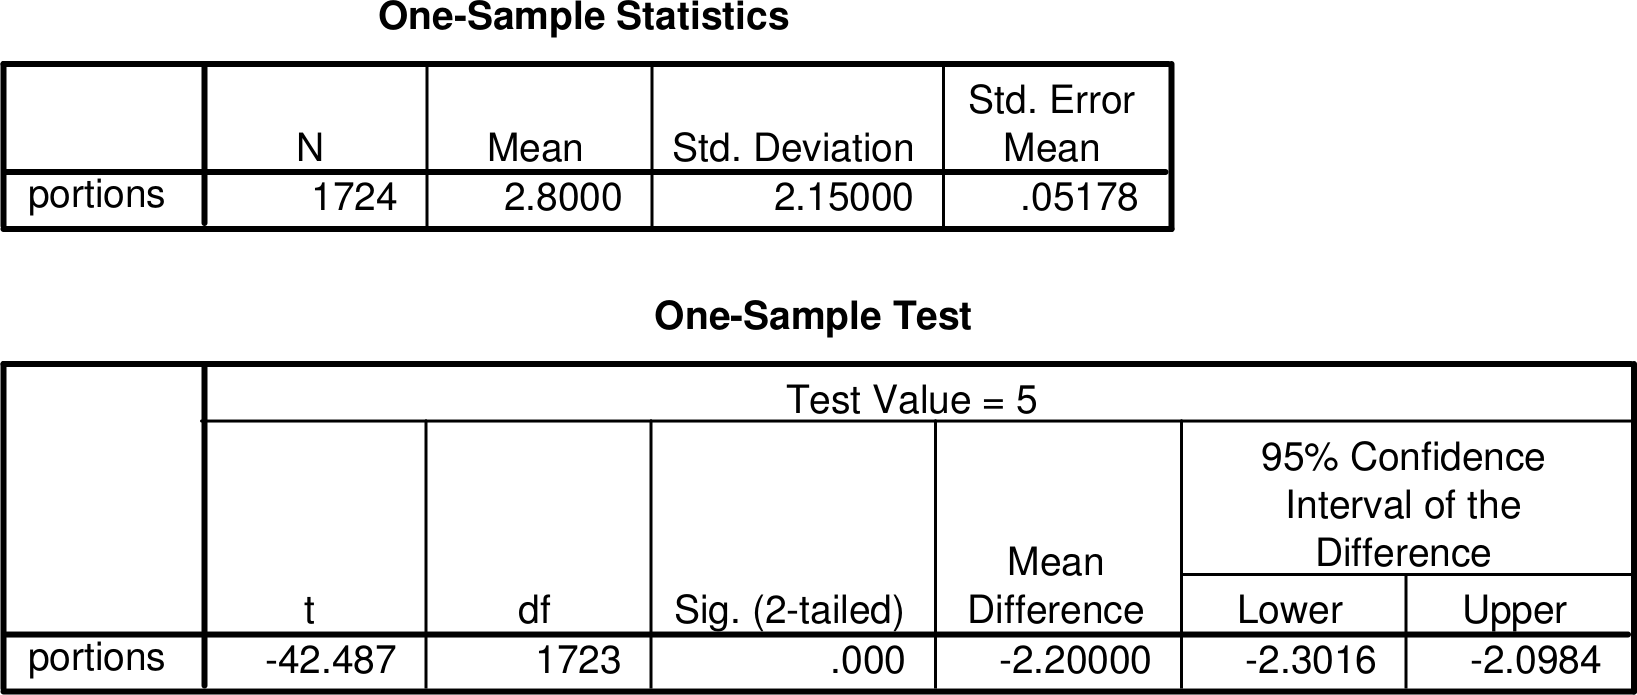
\includegraphics[bb=100 580 500 780, width=130mm]{ttestspss}
\end{figure}

Similar results for the variable on the percentage of dietary energy
obtained from fat are also shown in Table \ref{t_ttests1}. Here
$\mu_{0}=35$, $\hat{\Delta}=35.3-35=0.3$,
$\hat{\sigma}_{\hat{\Delta}}=6.11/\sqrt{1724}=0.147$, $t=0.3/0.147$, and
the two-sided $P$-value is $P=0.042$. Here $P<0.05$, so null hypothesis
that the population average of the percentage of energy obtained from
fat is 35 is rejected at the 5\% level of significance. However, because
$P>0.01$, the hypothesis would not be rejected at the next conventional
significance level of 1\%. The conclusions are the same if we considered
the one-sided alternative hypothesis $H_{a}:\; \mu>35$, for which
$P=0.042/2=0.021$ (as the observed sample mean $\bar{Y}=35.3$ is in the
direction of $H_{a}$). In this case the evidence against the null
hypothesis is thus somewhat less strong than for the fruit and vegetable
variable, for which the $P$-value was extremely small. The 95\%
confidence interval for the population average of the fat variable is
$35.3\pm 1.96\times 0.147=(35.01; 35.59)$.

Analysis of a single population mean is a good illustration of some of
the advantages of confidence intervals over significance tests. First, a
confidence interval provides a summary of all the plausible values of $\mu$
even when, as is very often the case, there is no obvious single value
$\mu_{0}$ to be considered as the null hypothesis of the one-sample
$t$-test. Second, even when such a significance test is sensible, the
conclusion can also be obtained from the confidence interval, as
discussed on page \pageref{p_civstest}. In other words, $H_{0}:\;
\mu=\mu_{0}$ is rejected at a given significance level against a
two-sided alternative hypothesis, if the confidence interval for $\mu$
at the corresponding confidence level does not contain $\mu_{0}$, and
not rejected if the interval contains $\mu_{0}$. Here the 95\%
confidence interval (2.70; 2.90) does not contain 5 for the fruit and
vegetable variable, and the interval (35.01; 35.59) does not contain 35
for the fat variable, so the null hypotheses with these values as
$\mu_{0}$ are rejected at the 5\% level of significance.

The width of a confidence interval also
gives information on how precise the results of the statistical analysis
are. Here the intervals seem quite narrow for both variables, in that it
seems that their end points (e.g.\ 2.7 and 2.9 for
portions of fruit and vegetables) would imply qualitatively similar
conclusions about the level of consumption in the population.
Analysis of the sample of 1724 respondents
in the National Diet and Nutrition Survey thus appears to have given us
quite precise information on the population averages for most practical
purposes. Of course, what is precise enough ultimately depends on what
those purposes are. If much higher precision was required, the sample
size in the survey would have to be correspondingly larger.

Finally, in cases where a null hypothesis is rejected by a significance
test, a confidence interval has the additional advantage of providing a
way to assess whether the observed deviation from the null hypothesis
seems large in some \emph{substantive} sense.
For example, the
confidence interval for the fat variable draws attention to the fact
that the evidence against a population mean of 35 is not very strong.
The lower bound of the interval is only 0.01 units above 35, which is
very little relative to the overall width (about 0.60) of the interval.
The $P$-value (0.041) of the test, which is not much below the reference
level of 0.05, also suggests this, but in a less obvious way. Even the
upper limit (35.59) of the interval is arguably not very far from 35, so
it suggests that we can be fairly confident that the population mean
does not differ from 35 by very much in the substantive sense. This
contrasts with the results for the fruit and vegetable variable, where
all the values covered by the confidence interval (2.70; 2.90) are much
more obviously far from the recommended value of 5.

%\renewcommand{\thefootnote}{\fnsymbol{footnote}}
\section{Inference for dependent samples}
%\footnote[1]{The material of this section is not required in the
%examination.}}
\label{s_means_dependent}
%\renewcommand{\thefootnote}{\arabic{footnote}}

In the two-sample cases considered in Section
\ref{s_means_inference}, the two groups being compared
consisted of separate and presumably unrelated units (people, in all of
these cases). It thus seemed justified to treat the groups as
statistically independent. The third and last general case considered in
this chapter is one where this assumption cannot be made, because there
are some obvious connections between the groups. Examples 7.4 and 7.5
(see page \pageref{p_dependentex}) illustrate this situation.
Specifically, in both cases we can find for each observation in one
group a natural \emph{pair} in the other group. In Example 7.4, the data
consist of observations of a variable for a group of fathers at two time
points, so the pairs of observations are clearly formed by the two
measurements for each father. In Example 7.5 the basic observations are
for separate days, but these are paired (\emph{matched}) in that for
each Friday the 13th in one group, the preceding Friday the 6th is
included in the other. In both cases the existence of the pairings
implies that we must treat the two groups as statistically
\emph{dependent}.

Data with dependent samples are quite common, largely because they are
often very informative. Principles of good research design suggest that
one key condition for being able to make valid
and powerful comparisons between two groups is that
the groups should be as similar as possible, apart from differing in the
characteristic being considered. Dependent samples represent an attempt
to achieve this through intelligent data collection.
In Example 7.4, the comparison of interest
is between a man's sense of well-being before and after the birth of his first
child. It is likely that there are also other factors which affect
well-being, such as personality and life circumstances
unrelated to the birth of a child. Here, however, we can compare the
well-being for the \emph{same} men before and after the birth, which
should mean that many of those other characteristics remain
approximately unchanged between the two measurements. Information on the
effects of the birth of a child will then mostly come not from overall levels
of well-being but \emph{changes} in it for each man.

In Example 7.5, time of the year and day of the week are likely to have
a very strong effect on traffic levels. Comparing, say, Friday, November
13th to Friday, July 6th, let alone to Sunday, November 15th, would thus
not provide much information about possible additional differences which
were due specifically to a Friday being the 13th. To keep these other
characteristics approximately constant and thus to focus on the effects
of Friday the 13th, each such Friday has here been matched with the
nearest preceding Friday. With this design, data on just ten
matched pairs will (as seen below) allow us to conclude that the
differences are statistically significant.

Generalisations of the research designs illustrated by Examples 7.4 and
7.5 allow for measurements at more than two occasions for each subject
(so-called longitudinal or panel studies) and groups of more than two
matched units (clustered designs). Most of these are
analysed using statistical methods which are  beyond the scope of
this course. The paired case is an exception, for which the analysis is
in fact easier than for two independent samples. This is because the
pairing of observations allows us to reduce the analysis into a
one-sample problem, simply by considering within-pair \emph{differences}
in the response variable $Y$. Only the case where $Y$ is a continuous
variable is considered here. There are also methods of inference for
comparing two (or more) dependent samples of response
variables of other types,
but they are not covered here.

The quantity of interest is again a population difference. This time it
can be formulated as $\Delta=\mu_{2}-\mu_{1}$, where $\mu_{1}$ is the
mean of $Y$ for the first group (e.g.\ the first time point in Example
7.4) and $\mu_{2}$ its mean for the second group. Methods of inference
for $\Delta$ will again be obtained using the same general results which
were previously applied to one-sample analyses and comparisons of two
independent samples. The easiest way to do this is now to consider a
new variable $D$, defined for each \emph{pair} $i$ as
$D_{i}=Y_{2i}-Y_{1i}$, where $Y_{1i}$ denotes the value of the first
measurement of $Y$ for pair $i$, and $Y_{2i}$ is the second measurement
of $Y$ for the same pair. In Example 7.4 this is thus the difference
between a man's well-being after the birth of his first baby, and the
same man's well-being before the birth. In Example 7.5, $D$ is the
difference in traffic flows on a stretch of motorway between a Friday
the 13th and the Friday a week earlier (these values are shown in the
last column of Table \ref{t_F13}). The number of observations of $D$ is
the number of pairs, which is equal to the sample sizes $n_{1}$ and
$n_{2}$ in each of the two groups (the case where one of the two
measurements might be missing for some pairs is not considered here). We
will denote it by $n$.

The population mean of the differences $D$ is also
$\Delta=\mu_{2}-\mu_{1}$, so the observed values $D_{i}$ can be used for
inference on $\Delta$. An estimate of $\Delta$ is the sample
average of $D_{i}$, i.e.\
\begin{equation}
\hat{\Delta}=\overline{D}=\frac{1}{n}\sum_{i=1}^{n} D_{i}.
\label{Dbar_dep}
\end{equation}
In other words, this is the average of the within-pair differences
between the two measurements of $Y$.
Its standard error is estimated by
\begin{equation}
\hat{\sigma}_{\hat{\Delta}} =
\frac{s_{D}}{\sqrt{n}}
\label{sDbar_dep}
\end{equation}
where $s_{D}$ is the sample standard deviation of $D$, i.e.\
\begin{equation}
s_{D} = \sqrt{\frac{\sum (D_{i}-\overline{D})^{2}}{n-1}}.
\label{s2D_dep}
\end{equation}
A test statistic for the null hypothesis $H_{0}: \Delta=0$
is given by
\begin{equation}
t=
\frac{\hat{\Delta}}{\hat{\sigma}_{\hat{\Delta}}}=
\frac{\overline{D}}{s_{D}/\sqrt{n}}
\label{zD_dep}
\end{equation}
and its $P$-value is obtained either from the standard normal
distribution or the $t_{n-1}$ distribution.
A confidence interval for $\Delta$ with confidence level $1-\alpha$
is given by
\begin{equation}
\hat{\Delta} \pm q_{\alpha/2} \times \hat{\sigma}_{\hat{\Delta}}
=\overline{D} \pm q_{\alpha/2} \times \frac{s_{D}}{\sqrt{n}}
\label{ciD_dep}
\end{equation}
where the multiplier $q_{\alpha/2}$ is either $z_{\alpha/2}$ or
$t_{\alpha/2}^{(n-1)}$. These formulas are obtained by noting
that this is simply a one-sample analysis
with the differences $D$ in place of the variable $Y$,
and applying the formulas of Section
\ref{s_means_1sample} to the observed values of $D$.

\begin{table}
\caption{Results of tests and confidence intervals for comparing
means of two dependent samples. For Example 7.4, the difference
is between after and before the birth of the child, and
for Example 7.5 it is between Friday the 13th and the preceding Friday
the 6th.
See the text for the
definitions of the statistics.}
\label{t_2tests_dep}

\begin{center}
\begin{tabular}{|rrrrr|}\hline
& & \multicolumn{2}{r}{Test of $H_{0}: \Delta=0$} & \\
$\hat{\Delta}$& $\hat{\sigma}_{\hat{\Delta}}$& $t$ & $P$-value &
95 \% C.I. for $\Delta$ \\ \hline
\multicolumn{5}{|l|}{Example 7.4: Father's personal well-being}\\
0.08 & 0.247 & 0.324 & 0.75$^{\dagger}$ & (-0.40; 0.56) \\
\hline
\multicolumn{5}{|l|}{Example 7.5: Traffic flows on successive
Fridays}\\
-1835 & 372 & -4.93 & 0.001$^{*}$ & (-2676; -994) \\
\hline
\multicolumn{5}{l}{{\footnotesize * Obtained from the $t_{9}$
distribution.}}\\
\multicolumn{5}{l}{{\footnotesize $\dagger$ Obtained from the
standard normal distribution.}}
\end{tabular}
\end{center}
\end{table}


Results for Examples 7.4 and 7.5 are shown in Table
\ref{t_2tests_dep}. To illustrate the calculations, consider Example
7.5. The $n=10$ values of $D_{i}$ for it are shown in Table \ref{t_F13},
and the summary statistics $\overline{D}=-1835$ and $s_{D}=1176$ in
Table \ref{t_groupex}. The standard error of $\overline{D}$ is thus
$s_{D}/\sqrt{n}=1176/\sqrt{10}=372$ and the value of the test
statistic (\ref{zD_dep}) is
\[
z=\frac{-1835}{1176/\sqrt{10}}=\frac{-1835}{372}=-4.93.
\]
This example differs from others we have considered so far in that the
sample size of $n=10$ is clearly too small for us to rely on
large-sample results. It is thus not appropriate to
refer the test statistic to a standard normal
distribution. Instead, $P$-values can be obtained from a
$t$ distribution, but only if the population distribution of $D$ itself
can be assumed to  be approximately normal. Here we have only
the ten observed values of $D$ to use for a rather informal assessment
of whether this assumption appears to be reasonable. One value of $D$ is
smaller than -4000, and 2, 5, 2 of them are in the ranges -3000 to
-2001, -2000 to -1001, and -1000 to -1 respectively. Apart from the
smallest observation, the sample distribution of $D$ is thus at least
approximately symmetric. While this definitely does not prove that $D$
is normally distributed, it is at least not obviously inconsistent with
such a claim. We thus feel moderately confident that we can apply here
tests
and confidence intervals based on the $t$ distribution.

The $P$-value, obtained from a $t$ distribution with $n-1=9$ degrees of
freedom, for the test statistic $-4.93$ is approximately 0.001. Even
with only ten pairs of observations, there is
significant evidence that the volume of traffic on a
Friday the 13th differs from that of the preceding Friday. A confidence
interval for the difference is obtained from (\ref{ciD_dep})
as
\[
-1835 \pm 2.26 \times 372 = (-2676; -994)
\]
where the multiplier 2.26 is the quantity
$t_{\alpha/2}^{(n-1)}=t_{0.975}^{(9)}$, obtained from a computer or a
table of the $t_{9}$-distribution. The interval shows that we are 95\%
confident that the average reduction in traffic on Friday the 13th on
the stretches of motorway considered here is between 994 and 2676
vehicles. This seems like a substantial systematic difference, although
not particularly large as a proportion of the total volume of traffic on
those roads. In the absence of other information we are tempted to
associate the reduction with some people avoiding driving on a day they
consider to be unlucky.

In Example 7.4 the $P$-value is 0.75, so we cannot reject the null
hypothesis that $\Delta=0$. There is thus no evidence that there was a
difference in first-time fathers' self-assessed level of well-being
between the time their wives were six months pregnant, and a month after
the birth of the baby. This is also indicated by the 95\% confidence
interval \mbox{($-0.40$; 0.56)} for the difference, which clearly covers the
value 0 of no difference.

\section{Further comments on significance tests}
\label{s_means_tests3}

Some further aspects of significance
testing are dicussed here. These are not practical issues that need to
be actively considered every time you carry out a test. Instead, they provide
context and motivation for the principles behind significance tests.

\subsection{Different types of error}
\label{ss_means_tests3_errors}

Consider for the moment the approach to significance testing where the
outcome is presented in the form of a discrete claim or
decision about the hypotheses, stating that the null hypothesis was
either rejected or not rejected. This claim can either be correct or
incorrect, depending on whether the null hypothesis is true in the
population. There are four possibilities, summarized in Table
\ref{t_twoerrors}. Two of these are correct decisions and two are
incorrect. The two kinds of incorrect decisions are traditionally called
\begin{itemize}
\item
\textbf{Type I error:} rejecting the null hypothesis when it is true
\item
\textbf{Type II error:} not rejecting the null hypothesis when it is
false
\end{itemize}
The terms are unmemorably bland, but they do at least suggest an order
of importance. Type I error is conventionally
considered more serious than Type II, so what we most want to avoid is
rejecting the null hypothesis unnecessarily. This implies that we will
maintain the null hypothesis unless data provide strong enough evidence
to justify rejecting it, a principle which is somewhat analogous to the
``keep a theory until falsified'' thinking of Popperian philosophy of
science, or even the ``innocent until proven guilty'' principle of
jurisprudence.

\begin{table}
\caption{The four possible combinations of the truth of a null hypothesis $H_{0}$ in a population and decision about it from a significance test.}
\label{t_twoerrors}
\begin{center}
\begin{tabular}{|ll|ll|}\hline
& & \multicolumn{2}{|c|}{$H_{0}$ is} \\
& & Not Rejected & Rejected \\  \hline
$H_{0}$ is & True & Correct decision & Type I error \\
& False & Type II error & Correct decision \\
\hline
\end{tabular}
\end{center}
\end{table}

Dispite our dislike of Type I errors, we will not try to avoid them
completely. The only way to guarantee that the null hypothesis is never
incorrectly rejected is never to reject it at all, whatever the
evidence. This is not a useful decision rule for empirical research.
Instead, we will decide in advance how high a probability of Type I
error we are willing to tolerate, and then use a test procedure with
that probability. Suppose that we use a 5\% level of significance to
make decisions from a test. The null hypothesis is then rejected if the
sample yields a test statistic for which the $P$-value is less than
0.05. If the null hypothesis is actually true, such values are, by the
definition of the $P$-value, obtained with probability 0.05. Thus the
significance level ($\alpha$-level) of a test is the probability of
making a Type I error. If we use a large $\alpha$-level (say
$\alpha=0.10$), the null hypothesis is rejected relatively easily
(whenever $P$-value is less than 0.10), but the chances of
committing a Type I
error are correspondingly high (also 0.10); with a smaller value like
$\alpha=0.01$, the error probability is lower because $H_{0}$ is
rejected only when evidence against it is quite strong.

This description assumes that the true probability of Type I error for a
test \emph{is} equal to its stated $\alpha$-level. This is true when the
assumptions of the test (about the population distribution, sample size
etc.) are satisfied. If the assumptions fail, the true significance
level will differ from the stated one, i.e.\ the $P$-value calculated
from the standard sampling distribution for that particular test will
differ from the true $P$-value which would be obtained from the exact
sampling distribution from the population in question. Sometimes the
difference is minor and can be ignored for most practical purposes (the
test is then said to be \emph{robust} to violations of some of its
assumptions). In many situations, however, using an inappropriate test
may lead to incorrect conclusions: for example, a test which claims that
the $P$-value is 0.02 when it is really 0.35  will clearly give a
misleading picture of the strength of evidence against the null
hypothesis. To avoid this, the task of statisticians is to develop valid
(and preferably robust) tests for many different kinds of hypotheses and
data. The task of the empirical researcher is to choose a test which is appropriate
for his or her data.

In the spirit of regarding Type I errors as the most serious, the worst
kind of incorrect test is one which gives too low a $P$-value, i.e.\
exaggerates the strength of evidence against the null hypothesis.
Sometimes it is known that this is impossible or unlikely, so that the
$P$-value is either correct or too high. The significance test is then
said to be \emph{conservative}, because its true rate of Type I errors
will be the same or lower than the stated $\alpha$-level. A conservative
procedure of statistical inference is regarded as the next best thing to
one which has the correct level of significance. For example, when the
sample size is relatively large, $P$-values for all of the tests
discussed in this chapter may be calculated from a standard normal or
from a $t$ distribution. $P$-values from a $t$ distribution are then
always somewhat larger. This means that using the $t$ distribution is
(very slightly) conservative when the population distributions are not
normal, so that we can safely use the $P$-values from SPSS output of a
$t$-test even in that case (this argument does not, however, justify
using the $t$-test when $Y$ is not normally distributed and the sample
size is small, because the sampling distribution of the $t$-test
statistic may then be very far from normal).

\subsection{Power of significance tests}
\label{ss_means_tests3_power}

After addressing the question of Type I error by selecting an
appropriate test and deciding on the significance level to be used, we
turn our attention to Type II errors. The probability that a
significance test will reject the null hypothesis when it is in fact not
true, i.e.\ the probability of \emph{avoiding} a Type II error, is known as the
\textbf{power} of the test. It depends, in particular, on
\begin{itemize}
\item
The nature of the test. If several valid tests are available for a
particular analysis, we would naturally prefer one which tends to have
the highest power. One aim of theoretical statistics is to identify the
most powerful test procedures for different problems.
\item
The sample size: other things being equal, larger samples mean higher power.
\item
The true value of the population parameter to be tested, here the
population mean or proportion. The power of any test will be highest
when the true value is very different from the value specified by the
null hypothesis. For example, it will obviously be easier to detect that
a population mean differs from a null value of $\mu_{0}=5$ when the true
mean is 25 than when it is 5.1.
\item
The population variability of the variable. Since large population
variance translates into large sampling variability and hence high
levels of uncertainty, the power will be low when population variability
is large, and high if the population variability is low.
\end{itemize}
The last three of these considerations are often used at the design
stage of a study to get an idea of the sample size required for a
certain level of power, or of the power achievable with a given sample
size. Since data collection costs time and money, we would not want to
collect a much larger sample than is required for a level of certainty
sufficient for the purposes of a study. On the other hand, if a
preliminary calculation reveals that the largest sample we can afford
would still be unlikely to give enough information to detect interesting
effects, the study might be best abandoned.

A power calculation requires the researcher to specify the kinds of
differences from a null hypothesis which are large enough to be of
practical or theoretical interest, so that she or he would want to be
able to detect them with high probability (it must always be accepted
that the power will be lower for smaller differences). For example,
suppose that we are planning a study to compare the effects of two
alternative teaching methods on the performance of students in an
examination where possible scores are between 0 and 100.
The null hypothesis is that average results are the same for students
taught with each method.
It is decided
that we want enough data to be able to reject this with high probability
if the true difference $\Delta$ of
the average exam scores between the two groups
is larger than 5
points, i.e.\ $\Delta<-5$ or $\Delta>5$.
The power calculation might then
answer questions like
\begin{itemize}
\item
What is the smallest sample size for which the probability of rejecting
$H_{0}: \Delta=0$ is at least 0.9,
when the true value of $\Delta$ is smaller than $-5$ or
larger than 5?
\item
The largest sample sizes we can afford are 1000 in both groups, i.e.\
$n_{1}=n_{2}=1000$. What is the probability this gives us of rejecting
$H_{0}: \Delta=0$ when the true value of $\Delta$ is smaller than $-5$
or larger than 5?
\end{itemize}
To answer these questions, we would also need a rough guess of the
population standard deviations $\sigma_{1}$ and $\sigma_{2}$, perhaps
obtained from previous studies. Such calculations employ further
mathematical results for test statistics, essentially using their
sampling distributions under specific alternative hypotheses. The
details are, however, beyond the scope of this course.

\subsection{Significance vs.\ importance}
\label{ss_means_tests3_importance}

The $P$-value is a measure of the strength of evidence the data provide
against the null hypothesis. This is not the same as the magnitude of
the difference between sample estimates and the null hypothesis, or
the practical importance of such differences. As noted above, the power of a
test increases with increasing sampling size. One implication of this is
that when $n$ is large, even quite small observed deviations from the
values that correspond exactly to the null hypothesis will be judged to
be statistically significant. Consider, for example, the two dietary
variables in Table
\ref{t_ttests1} on page
\pageref{t_ttests1}.
The sample mean of the fat variable is 35.3, which is significantly
different (at the 5\% level of significance) from $\mu_{0}$ of 35. It is
possible, however, that a difference of 0.3 might be considered
unimportant in practice. In contrast, the sample mean of the fruit and
vegetable variable is 2.8, and the difference from $\mu_{0}$ of 5 seems
not only strongly significant but also large for most practical
purposes.

In contrast to the large-sample case, in small samples even quite large
apparent deviations from the null hypothesis might still result in a
large $P$-value. For example, in a very small study a sample mean of the
fat variable of, say, 30 or even 50 might not be interpreted as sufficiently
strong evidence against a population mean of 35. This is obviously
related to the discussion of statistical power in the previous section,
in that it illustrates what happens when the sample is too small to
provide enough information for useful conclusions.

In these and all other cases, decisions about what is or is not of
practical importance are subject-matter questions rather than statistical ones,
and would have to be based on information about the nature and
implications of the variables in question. In our dietary examples this
would involve at least medical considerations, and perhaps also
financial implications of the public health costs of the observed
situation or of possible efforts of trying to change it.
